% Build: xelatex -interaction=nonstopmode -halt-on-error Ariadne_0_8_0_Textbook.tex
% Run three times from this directory. Figures and subset open fonts are included.
\documentclass[11pt,oneside,openany]{book}
\usepackage[a4paper,margin=24mm,headheight=15pt,footskip=12mm]{geometry}
\usepackage{fontspec}
\setmainfont[Path=fonts/,BoldFont=ReportSerif-Bold.ttf]{ReportSerif-Regular.ttf}
\setsansfont[Path=fonts/,BoldFont=ReportSans-Bold.ttf]{ReportSans-Regular.ttf}
\setmonofont{Latin Modern Mono}[Scale=0.86]
\newfontfamily\latintext{Latin Modern Roman}
\XeTeXlinebreaklocale "zh"
\XeTeXlinebreakskip=0pt plus 0.08em
\usepackage{amsmath,amssymb,mathtools,bm,amsthm}
\usepackage{graphicx,booktabs,longtable,tabularx,array}
\usepackage{xcolor,enumitem,fancyhdr,titlesec}
\usepackage{tikz}
\usetikzlibrary{arrows.meta,positioning,calc,fit,shapes.geometric}
\usepackage[unicode,colorlinks=true,linkcolor=blue!35!black,citecolor=blue!35!black,urlcolor=blue!50!black]{hyperref}
\usepackage{listings}
\definecolor{ink}{HTML}{1D354D}
\definecolor{accent}{HTML}{B86937}
\definecolor{pale}{HTML}{F2F5F7}
\titleformat{\chapter}[display]{\Large\bfseries\color{ink}}{\large 第\thechapter 章}{7pt}{\huge}
\titlespacing*{\chapter}{0pt}{-8pt}{20pt}
\titleformat{\section}{\large\bfseries\color{ink}}{\thesection}{0.7em}{}
\titleformat{\subsection}{\normalsize\bfseries}{\thesubsection}{0.6em}{}
\renewcommand{\contentsname}{目录}
\renewcommand{\bibname}{参考文献}
\renewcommand{\figurename}{图}
\renewcommand{\tablename}{表}
\renewcommand{\appendixname}{附录}
\setcounter{tocdepth}{1}
\setcounter{secnumdepth}{2}
\setlength{\parindent}{2em}
\setlength{\parskip}{3pt}
\linespread{1.12}
\setlist{itemsep=3pt,topsep=5pt,leftmargin=2em}
\pagestyle{fancy}\fancyhf{}
\fancyhead[L]{\small Ariadne：从衍射像素到晶体结构}
\fancyhead[R]{\small 原理与实现 · 0.8.0}
\fancyfoot[C]{\thepage}
\renewcommand{\headrulewidth}{0.3pt}
\newcommand{\code}[1]{\texttt{\detokenize{#1}}}
\newcommand{\dif}{\mathrm{d}}
\newcommand{\iu}{\mathrm{i}}
\newcommand{\E}{\mathbb{E}}
\newcommand{\Var}{\operatorname{Var}}
\newcommand{\Cov}{\operatorname{Cov}}
\newcommand{\rank}{\operatorname{rank}}
\newcommand{\diag}{\operatorname{diag}}
\newcommand{\argmin}{\operatorname*{arg\,min}}
\newcommand{\angstrom}{\text{\AA}}
\newenvironment{worked}[1]{\begin{quote}\small\textbf{例：#1}\par}{\end{quote}}
\newenvironment{principle}{\begin{quote}\small\color{ink}}{\end{quote}}
\lstset{basicstyle=\footnotesize\ttfamily,breaklines=true,frame=single,rulecolor=\color{black!15},backgroundcolor=\color{pale},columns=fullflexible,keepspaces=true,showstringspaces=false}
\renewcommand{\topfraction}{0.9}\renewcommand{\bottomfraction}{0.85}
\renewcommand{\textfraction}{0.08}\renewcommand{\floatpagefraction}{0.75}
\emergencystretch=3em\allowdisplaybreaks
\hypersetup{pdftitle={Ariadne 0.8.0：从衍射像素到晶体结构——数学、算法与原生智能体},pdfauthor={Ariadne technical documentation}}
\setlength{\intextsep}{8pt}\setlength{\textfloatsep}{12pt}

\begin{document}
\frontmatter
\begin{titlepage}
\vspace*{12mm}
\noindent{\large\sffamily\color{accent} ARIADNE · 技术教材}\par
\vspace{16mm}
\noindent{\Huge\bfseries 从衍射像素\\[7pt]到晶体结构}\par
\vspace{12mm}
\noindent{\Large 数学、算法与原生智能体}\par
\vspace{15mm}
\noindent\rule{\textwidth}{0.8pt}\par
\vspace{4mm}
\noindent{\large 直接法\quad 双空间求解\quad 像素似然\quad 联合精修}\par
\vspace{14mm}
\begin{tikzpicture}[node distance=11mm, every node/.style={font=\small}, box/.style={draw=ink!50,rounded corners=2pt,fill=pale,minimum height=13mm,text width=27mm,align=center}, >=Latex]
\node[box] (p) {像素与几何};
\node[box,right=of p] (l) {可测的强度组合};
\node[box,right=of l] (s) {结构候选};
\node[box,right=of s] (v) {独立验证};
\draw[->,thick,ink] (p)--(l);\draw[->,thick,ink] (l)--(s);\draw[->,thick,ink] (s)--(v);
\draw[->,thick,accent] (s.south) -- ++(0,-12mm) -| node[pos=0.2,below]{用结构预测检验像素解释} (p.south);
\end{tikzpicture}
\vfill
\noindent{\large Ariadne 0.8.0 · 研究版}\par
\vspace{3mm}
\noindent 2026 年 11 月 8 日\par
\vspace{4mm}
\noindent\small 基于可核对的 Ariadne 0.7.0 与 Ariadne-Xtal 0.1.0 源码重构。\\
本书对应随附源代码、可重复实验脚本和本次运行的验证记录。
\end{titlepage}

\chapter*{读者指南}
\addcontentsline{toc}{chapter}{读者指南}
本书回答一个实际问题：能否把单晶衍射的数据还原、相位求解、结构精修和自动决策放在同一个数学框架里，使弱衍射和孪晶得到更合理的处理？答案是可以，但连接这些步骤的对象必须是观测似然及其不确定度。把某个模型预测的强度写回成“测得的强度”，会使结构看起来越来越正确，却没有增加实验信息。

阅读顺序从波的叠加开始。第一至四章解释反射如何形成、怎样预测它落在哪个像素、怎样从有噪声和重叠的像素中取得信息，以及如何缩放和导出。第五、六章讲相位问题、直接法、双空间迭代和原点与空间群。第七、八章把精修写成可求导的物理模型，并把重叠像素直接接到结构参数上。第九章说明智能体怎样利用这些模块形成可检验的闭环。第十、十一章讲 C++ 数值内核和资源约束任务调度，最后两章给出源码接口、实测结果和使用方法。

\begin{principle}
“替代 SHELXT/SHELXL”在本项目中指逐步建立独立的原生计算内核。0.8.0 已能在明确适用的输入上独立完成相位求解、结构精修和重叠观测联合拟合；完整 SHELX 指令语言、所有自动结构处理和所有仪器的端到端生产验证，仍有专门的工程范围。第\ref{chap:software}章逐项列出当前实现。
\end{principle}

本次工作保留 Ariadne 原有 DIALS 适配、几何与体素积分、缩放、导出、进程隔离和持久化智能体能力。新增内容集中在有实质计算差异的环节：强度似然驱动的混合相位更新、带原点的对称投影、解析精修导数、保留重叠信息的结构精修，以及分离生成、选择和最终验证的原生流程。

本书中的图分为三类：由公式直接计算的教学图；有指定随机种子的合成数据实验；公开 FeN$_4$ 实验强度的已知模型再精修。图注均标明来源。没有将合成数据的误差当作真实 MOF 的成功率，也没有使用 SHELXT/SHELXL 的运行结果冒充本软件的计算结果。

\begingroup\small\setlength{\parskip}{0pt}\linespread{0.96}\selectfont\tableofcontents\endgroup
\chapter*{统一记号}
\addcontentsline{toc}{chapter}{统一记号}
\begin{longtable}{p{0.25\textwidth}p{0.68\textwidth}}
\toprule 记号 & 含义与单位\\\midrule
$A, B=A^{-\mathsf T}$ & 正、倒易基矢矩阵；列为基矢；单位分别为 $\angstrom$、$\angstrom^{-1}$。\\
$x,r=Ax$ & 原子的分数坐标与笛卡尔坐标。\\
$h=(h,k,l)^{\mathsf T}$ & Miller 指数列向量；代码批量存储为行。\\
$q=Bh$ & 不含 $2\pi$ 的倒易矢量；$s=\|q\|/2=\sin\theta/\lambda$。\\
$F_h,I_h$ & 复结构因子与物理衍射强度；$I_h\propto |F_h|^2$。\\
$y,\sigma^2$ & 含噪观测及其方差；背景扣除后的 $y$ 可以为负。\\
$P,B_g$ & 像素轮廓矩阵和背景基矩阵；$B_g$ 与倒易基 $B$ 区分。\\
$R,z,c$ & 高斯像素压缩后的矩阵、目标和与结构参数无关的残差常数。\\
$U_j,o_j$ & 位移协方差张量（$\angstrom^2$）与物理位置占有率。\\
$\theta,\alpha$ & 结构的独立参数与各晶畴的非负比例，$\sum_d\alpha_d=1$。\\
$J,H$ & 残差 Jacobian 与局部信息矩阵；通常 $H=J^{\mathsf T}J$。\\
\code{work/selection/audit} & 候选拟合、候选选择、最后一次独立评价的数据角色。\\
\bottomrule
\end{longtable}
\mainmatter
\chapter{从波的叠加到一个反问题}
\section{探测器测到了什么}
设入射、出射波矢分别为 $k_0,k_1$，采用不含 $2\pi$ 的约定，$\|k_0\|=\|k_1\|=1/\lambda$。位于 $r$ 的一个电子相对于原点产生相位差 $2\pi(k_1-k_0)\cdot r$。晶胞电子密度为 $\rho(r)$ 时，散射振幅是各位置的复振幅之和：
\begin{equation}
 F(q)=\int_{\text{cell}}\rho(r)\exp(2\pi\iu q\cdot r)\,\dif r,
 \qquad q=k_1-k_0 .
\end{equation}
晶格的周期重复使这些波只在倒易晶格附近相长叠加。令 $q=Bh$、$r=Ax$，因为 $B^{\mathsf T}A=I$，有 $q\cdot r=h\cdot x$。这就是 Miller 指数和分数坐标能直接出现在相位里的原因。

普通 X 射线探测器统计到达的光子或由它们形成的电荷，没有记录波的相位。理想衍射强度与 $|F_h|^2$ 成正比，但原始像素还包含背景、有限峰宽、几何因子、吸收和探测器噪声。软件的基本任务因此是反推一组能够产生这些像素的物理参数。

\section{原子模型与温度因子}
若电子密度是各原子电子云的叠加，原子发生均值为零、协方差为 $U_j$ 的高斯位移，则位移的特征函数给出
\begin{equation}
 \E\{\exp(2\pi\iu q\cdot u_j)\}=\exp(-2\pi^2q^{\mathsf T}U_jq).
\end{equation}
定义 $s=\sin\theta/\lambda=\|q\|/2$，其中 $2\theta$ 是散射角；$s$ 与 $q$ 的单位均为倒数长度。因此结构因子可以写为
\begin{equation}\label{eq:structure-factor}
 F_h(\theta)=\sum_j\sum_{o\in G/H_j}o_j
 \left[f^0_j(s)+f'_j+\iu f''_j\right]
 \exp\!\left[-2\pi^2q^{\mathsf T}U_{jo}q+2\pi\iu h^{\mathsf T}x_{jo}\right].
\end{equation}
$G$ 是空间群，$H_j$ 是保持位置 $j$ 不变的稳定子群。商 $G/H_j$ 的作用是只对不同的物理位置求和。一个位于反演中心、完整占据的原子，占有率仍是 1；不能因为若干对称操作得到同一位置，就把它重复计数或任意修改占有率。

当 $U_j=u_jI$ 时，指数退化为 $-8\pi^2u_js^2$。非球形热运动则必须保留张量。旋转对称操作也要旋转张量；只旋转坐标、保持各向异性张量不动，会在高角反射中产生系统误差。

本包用 Gemmi 提供的 IT92 中性原子散射系数和空间群表，自行计算式\eqref{eq:structure-factor}及其导数。$f'$、$f''$ 是显式输入，不把波长依赖或反常散射自动猜进去。这里采用运动学 X 射线模型；多重散射强烈的电子衍射需要额外的前向模型。

\section{相干叠加与孪晶的非相干叠加}
同一有序晶胞内的原子先加振幅，再取平方；通常的宏观孪晶畴之间采用非相干强度混合：
\begin{equation}\label{eq:twin-intensity}
 \mu_h=k\sum_{d=1}^{D}\alpha_d\,|F_{T_dh}(\theta)|^2,
 \quad \alpha_d\ge0,\quad\sum_d\alpha_d=1.
\end{equation}
两种求和顺序不能互换。$|F_1+F_2|^2$ 含有干涉交叉项，通常不能用于描述独立孪晶畴的完全重叠。对于非面网孪晶，某个探测器区域可能只重叠一部分反射；这时每个分量有自己的索引和像素轮廓，应回到更一般的模型
\begin{equation}\label{eq:pixel-forward}
 \mu_i=b_i+\sum_j P_{ij}(\eta)c_j(\eta)\alpha_{d(j)}k|F_{h_j}(\theta)|^2 .
\end{equation}
$\eta$ 包含仪器几何与轮廓参数，$c_j$ 包含已经明确的相对标度与校正因子。式\eqref{eq:pixel-forward}将像素处理与结构精修接成了同一个问题。

\section{信息在哪一步丢失}
把像素压缩成强度表并不一定丢失有用信息。关键在于保留的数据是否足以对所有候选结构计算同一个似然。固定方差的线性高斯模型存在精确的有限维压缩；一般泊松像素模型则不能随意压成一个强度和一个标准差。

相位丢失是另一件事。设 $F_h=|F_h|e^{\iu\phi_h}$，在不改变 $|F_h|$ 的情况下改变相位，可以得到完全不同的电子密度。图\ref{fig:phase-basic}展示了这一点。相位求解必须引入原子性、密度约束、对称性或化学组成等额外信息。
\begin{figure}[!htbp]
\centering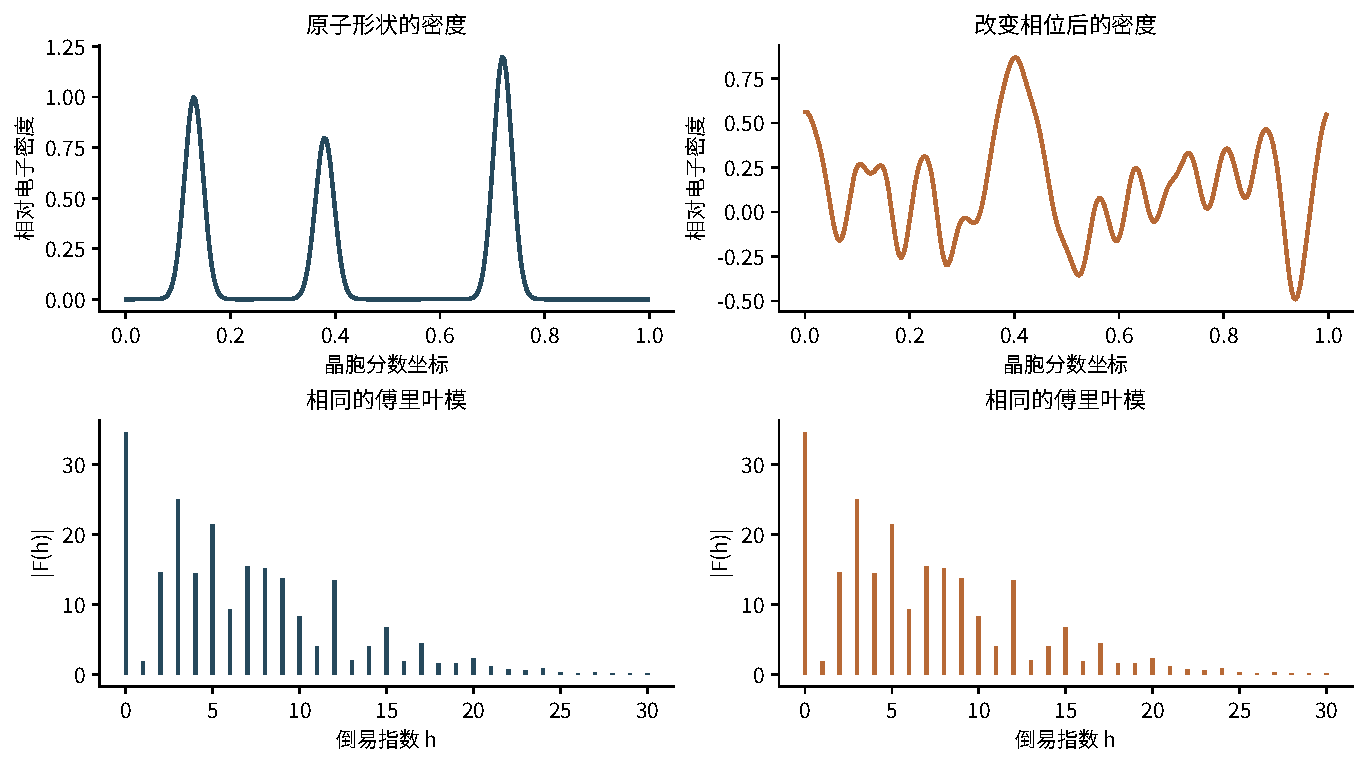
\includegraphics[width=\textwidth]{figures/01_phase_problem.pdf}
\caption{一维教学模型。两组傅里叶系数具有相同的模，但相位不同，得到的实空间密度明显不同。上方的原子峰与下方的相位扰动密度都由随附绘图脚本直接计算；它们不是实验数据。}\label{fig:phase-basic}
\end{figure}

\begin{principle}
从像素到结构的每一步都应回答两个问题：前向模型是什么？哪些未知量能由当前数据区分？速度优化只有在不改变这两个问题的含义时，才是可靠的优化。
\end{principle}

\chapter{从倒易点到探测器体素}
\label{chap:geometry}

\section{反射预测是一道几何方程}

一张衍射图记录的是散射光子到达探测器的位置。要把一个斑点解释为
$(h,k,l)$，必须同时满足晶格、转动和探测器几何。设实空间晶胞矩阵
$A_{\mathrm d}$ 的列为晶格矢量，长度单位为 \AA；取不含 $2\pi$ 的倒易约定，
\begin{equation}
 B=A_{\mathrm d}^{-T},\qquad
 \bm q=UB\bm h,\qquad d_{hkl}^{-1}=\|\bm q\|.
 \label{eq:geometry-reciprocal}
\end{equation}
这里 $U$ 是晶体取向，$\bm h=(h,k,l)^T$；$\bm q$ 的单位为
\AA$^{-1}$。散射矢量的定义必须与波矢保持一致，不能把含 $2\pi$ 和不含
$2\pi$ 的约定混用。

设入射波矢为 $\bm s_0$，其长度是 $1/\lambda$。测角仪将倒易点转到
$\bm r(\phi)$；用 $G_{\mathrm f}$、$G_{\mathrm s}$ 分别表示固定与设置转动，
则弹性散射要求
\begin{equation}
 \bm r(\phi)=G_{\mathrm s}R_{\bm e}(\phi)G_{\mathrm f}UB\bm h,
 \qquad
 \bm s_1=\bm s_0+\bm r,\qquad
 2\bm s_0^T\bm r+\|\bm r\|^2=0.
 \label{eq:geometry-ewald}
\end{equation}
最后一个等式就是 Ewald 球条件。它决定反射出现的转角，而不是在图上寻找一个
足够近的点就算预测成功。Ariadne 沿用 DIALS 的反射枚举、进入／离开球面的分支、
探测器面板及扫描周次选择\cite{dials2018}。

\begin{figure}[!htbp]
 \centering
 \begin{tikzpicture}[scale=0.95]
  \begin{scope}
   \draw[gray] (-1.6,0) circle (1.6);
   \fill (-1.6,0) circle (1.3pt) node[below] {$C$};
   \fill (0,0) circle (1.3pt) node[below right] {$O$};
   \fill (-0.8,1.386) circle (1.5pt) node[above right] {倒易点};
   \draw[->,thick] (-1.6,0)--(0,0) node[midway,below] {$\bm s_0$};
   \draw[->,thick] (-1.6,0)--(-0.8,1.386) node[midway,left] {$\bm s_1$};
   \draw[->,thick] (0,0)--(-0.8,1.386) node[midway,right] {$\bm r$};
   \node at (-1.6,-2.05) {倒易空间：波矢长度不变};
  \end{scope}
  \begin{scope}[xshift=4.9cm]
   \fill (0,0) circle (1.5pt) node[below] {晶体};
   \draw[thick] (2.9,-0.25)--(2.9,2.25) node[above] {探测器平面};
   \draw[->,thick] (0,0)--(2.9,1.35) node[midway,above] {$\widehat{\bm s}_1$};
   \fill (2.9,1.35) circle (1.5pt) node[right] {$\bm x$};
   \draw[dashed] (0,0)--(2.9,0);
   \draw[->] (2.9,0)--(2.9,1.3) node[midway,right] {$X$};
   \node at (1.4,-2.05) {实验空间：射线与面板相交};
  \end{scope}
 \end{tikzpicture}
 \caption{同一条反射的两种几何描述。左图中的长度为倒易长度，右图中的位置为实际长度；
 示意图没有表达晶胞或仪器的具体尺寸。}
 \label{fig:geometry-ewald-ray}
\end{figure}

\section{位置导数与仪器单位}

局部优化不必为每个参数反复搜索整个 Ewald 球。对已经选定的物理解作隐式微分，
记 $\bm t=(G_{\mathrm s}\bm e)\times\bm r$，可得
\begin{equation}
 \frac{\partial\phi}{\partial p}
 =-\frac{\bm s_1^T(\partial\bm r/\partial p)_{\phi}}
          {\bm s_0^T\bm t}.
 \label{eq:geometry-phi-derivative}
\end{equation}
分母趋近零对应切触情形，此时很小的晶体扰动也会引起很大的转角变化。
保留的解析导数代码显式检查这种退化，不用任意有限差分步长掩盖它。

探测器面板由原点 $\bm o$、法向 $\bm n$ 和面内单位轴
$\bm e_x,\bm e_y$ 描述。令 $\widehat{\bm s}_1$ 为单位出射方向，则
\begin{equation}
 \ell=\frac{\bm n^T\bm o}{\bm n^T\widehat{\bm s}_1},\qquad
 \bm x=\ell\widehat{\bm s}_1,\qquad
 X=\bm e_x^T(\bm x-\bm o),\quad
 Y=\bm e_y^T(\bm x-\bm o).
 \label{eq:geometry-detector}
\end{equation}
$\bm o,\ell,X,Y$ 使用 mm，之后才用像素尺寸换算为像素坐标。
扫描角使用 rad；若每帧角宽为 $\Delta\phi$，帧坐标为
$(\phi-\phi_0)/\Delta\phi$。沿用代码的质心残差是
$(\Delta X,\Delta Y,\Delta\phi)$，并非三个具有相同单位的长度。

取向属于旋转群，局部扰动可以写成
\begin{equation}
 U_{\mathrm{new}}=\exp([\delta\bm\omega]_\times)U,
 \qquad \delta\bm q=\delta\bm\omega\times\bm q+O(\|\delta\bm\omega\|^2).
 \label{eq:geometry-so3}
\end{equation}
这说明应在旋转切空间上优化，而不是把九个矩阵元素独立调整。
现有 DIALS 适配器使用保持晶体对称性的 $U/B$ 参数化，本次没有另造仪器标定器。

几何也有可辨识性边界。例如波长和晶胞长度同比例改变时，衍射角可以保持不变。
因此需要固定有独立标定依据的量，并检查残差随扫描角、面板和分辨率的系统变化。
增加自由参数通常能降低质心残差，却不一定更接近真实仪器。

几何误差还会改变似然的宽度。在线性近似下，若几何参数协方差为 $\Sigma_g$，
\begin{equation}
 C_i=C_{i,\mathrm{centroid}}+J_i\Sigma_gJ_i^T,
 \qquad C_{ij}^{\mathrm{shared}}=J_i\Sigma_gJ_j^T.
 \label{eq:geometry-covariance}
\end{equation}
第二项提醒我们：同一仪器误差可以同时移动许多反射。现有单源质心 EM 可以白化完整
$3\times3$ 观测协方差，但共同仪器固定；声明的模型协方差不等于已经求得全部仪器参数误差。
像素中的局部位置扰动消元，也应与整台仪器的共享协方差区分。

\section{探测器记录体素积分}

一个像素在一帧内积累的是有限体积上的概率质量。若三维轮廓密度为
$g(\bm u-\bm c;\Sigma)$，则
\begin{equation}
 P_{ij}=\int_{\Omega_i}g_j(\bm u-\bm c_j;\Sigma_j)\,d^3\bm u,
 \qquad \mu_i=b_i+\sum_j I_jP_{ij}.
 \label{eq:geometry-voxel}
\end{equation}
这里 $\bm u$ 使用两个像素坐标和一个帧坐标，$P_{ij}$ 无量纲，$I_j$ 是完整轮廓强度。
因此裁切盒内 $\sum_iP_{ij}<1$ 是正常的；不能再次归一化后又除一次 partiality。
体素中心的密度乘体积仅是近似，窄斑点或像素边界附近尤其需要真正积分。

对角 Gaussian 轮廓可精确分离为三个一维 CDF 差：
\begin{equation}
 P_i=\prod_{a=1}^{3}\left[
 \Phi\!\left(\frac{u_{ia}^{+}-c_a}{\sigma_a}\right)
 -\Phi\!\left(\frac{u_{ia}^{-}-c_a}{\sigma_a}\right)\right].
 \label{eq:geometry-cdf}
\end{equation}
相关轮廓的沿用实现解析积分一个条件正态方向，其余方向使用分块
Gauss--Legendre 积分。节点规则是数值精度策略，并非严格的误差证明。
平移导数则由体素表面的通量得到：
\begin{equation}
 \frac{\partial P_i}{\partial c_a}
 =\int_{\partial\Omega_{i,a}^{-}}g\,dS
  -\int_{\partial\Omega_{i,a}^{+}}g\,dS.
 \label{eq:geometry-face-flux}
\end{equation}
相邻体素共用的内表面通量相消，因此导数与质量守恒一致，也省去了反复平移后的体积分。

\section{强参考与弱数据各自承担什么任务}

分离清楚、定位稳定且覆盖扫描角的参考斑点适合约束几何和学习轮廓。
局部模板由参考数据向全局模板收缩，并使用非负三线性插值；校准范围外回到全局模板。
这比给每个弱斑点另拟合一套宽度更容易控制方差。
沿用实现采用的收缩规则为
\begin{equation}
 \widehat g_{\mathrm{local}}=
 \frac{n}{n+\kappa}\overline g_{\mathrm{local}}
 +\frac{\kappa}{n+\kappa}\overline g_{\mathrm{pooled}},
 \qquad n>0,\ \kappa>0.
 \label{eq:geometry-profile-shrinkage}
\end{equation}
$n$ 是当地有效参考数，$\kappa$ 控制向共享模板收缩的程度。
参考少时依靠全局形状，参考充分时才允许局部变化；这里约束的是轮廓形状，不是把弱反射的强度拉向某个目标值。

参考子集只服务于初始化和标定，不自动成为最终积分的删点规则。
一个重叠质心不能复制成多个独立观测；单源 EM 处理的是来源不确定性，复合斑点应回到共同像素模型。
0.8 的新接口接收上述轮廓，再按计数模型和可辨识性保留弱信号及重叠组合量。
几何比较沿用扫描块留出，使训练与检查覆盖不同角度区域。它评估的是给定候选的预测能力，
不能自动声称候选生成过程也完全独立；模型选择应同时查看剩余未解释斑点和各域的独立锚点。

\begin{table}[!htbp]
 \centering\small
 \caption{本章数学对象与沿用的源码。路径前缀为
 \code{skills/ariadne-reduction/scripts/}。}
 \begin{tabularx}{\textwidth}{@{}p{0.39\textwidth}X@{}}
  \toprule
  模块 & 实际职责 \\
  \midrule
  \code{rotation_geometry.py} & 已选反射分支的解析位置导数与白化距离。\\
  \code{centroid_em.py} & 固定仪器下的单源质心 EM、DIALS $U/B$ 适配。\\
  \code{profile_geometry.py} & 三维 Gaussian 体素概率与面通量导数。\\
  \code{profile_learning.py} & 有限工作内存的模板对齐、汇总及收缩。\\
  \code{local_profiles.py} & 固定局部模板的非负插值。\\
  \bottomrule
 \end{tabularx}
\end{table}

这些模块来自保留的 0.7 数值优化。0.8 的新增工作是将它们产生的前向设计接到原生像素似然和结构精修；
本次合成数值验证不等同于完成某台仪器原始帧的端到端标定与还原。

\chapter{弱衍射和重叠：先写对似然}
\section{负强度并不意味着负光子}
若背景扣除后的观测满足 $y\sim\mathcal N(I,\sigma^2)$，即使物理信号 $I\ge0$，也可能测得 $y<0$。对于 $I=0$，
\begin{equation}
 \E(y)=0,\qquad \E\{\max(y,0)\}=\frac{\sigma}{\sqrt{2\pi}}.
\end{equation}
所以把所有负观测裁成零会人为增加弱反射的平均信号。若进一步只保留 $y/\sigma$ 大的行，入选样本还会偏向正噪声。French--Wilson 方法讨论的是如何结合统计先验估计振幅，而不是允许把先验后的振幅当成新的独立测量\cite{french1978}。

本软件在 $F^2$ 精修中保留所有有效的带符号强度。相位初始化可以构造非负振幅作为数值起点，但新的混合算法随后使用原始 $y,\sigma$ 的强度似然。真实光子计数则使用非负计数模型，两者的“非负”作用于不同对象。
\begin{figure}[!htbp]
\centering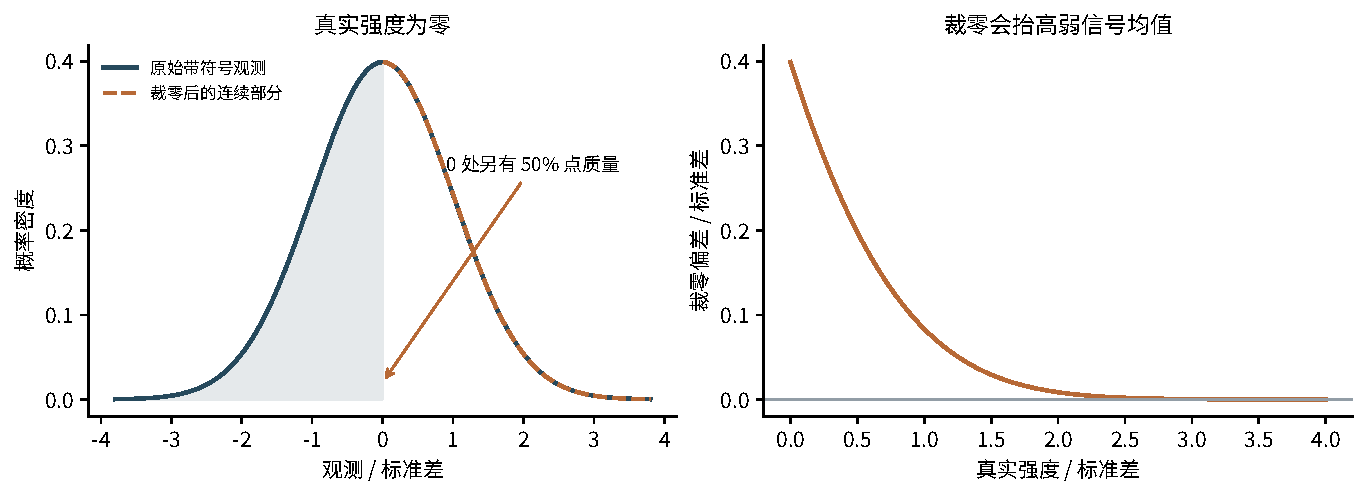
\includegraphics[width=0.94\textwidth]{figures/03_weak_bias.pdf}
\caption{零真实信号的高斯教学模型。负观测是噪声模型的一部分；裁零后在原点形成点质量，均值由零变为 $0.399\sigma$。右侧展示不同真实信号下裁零估计的偏差。曲线来自解析公式，不是软件成功率。}
\end{figure}

\section{高斯像素的背景消元}
令同一像素组内的模型为
\begin{equation}
 y=PI+B_g\beta+\varepsilon,\qquad \varepsilon\sim\mathcal N(0,W^{-1}).
\end{equation}
$I$ 是所有反射分量的强度，$B_g\beta$ 是共同背景。白化后 $\widetilde y=W^{1/2}y$、$\widetilde P=W^{1/2}P$。若 $Q_b$ 的列张成 $W^{1/2}B_g$，消去线性背景等价于
\begin{equation}
 \min_\beta\|W^{1/2}(y-PI-B_g\beta)\|^2
 =\|(I-Q_bQ_b^{\mathsf T})(\widetilde y-\widetilde PI)\|^2.
\end{equation}
实现中不显式生成像素数平方的投影矩阵。对增广设计矩阵按行分块作 QR 消元，再对小矩阵分解，可得到
\begin{equation}\boxed{\quad\chi^2(I)=\|RI-z\|^2+c.\quad}\label{eq:sufficient}
\end{equation}
$R,z,c$ 对任意候选 $I$ 都保留相同目标值。$c$ 不影响最优结构，却影响完整的拟合统计；比较模型或报告像素残差时不能丢掉它。这种方法属于可分离变量消元与平方根最小二乘的应用\cite{golub1973}。

QR 的价值还在于避免先形成 $P^{\mathsf T}WP$。后者将条件数平方；高度重叠时，浮点误差会更早破坏最弱的信息方向。新接口同时保留小矩阵、零空间和原始强度单位。

\section{可辨识性比强弱更基本}
对两个形状完全相同的峰，$P=[p,p]$，像素只依赖 $I_1+I_2$。无论曝光多少次，都不能仅靠这组像素区分 $(I_1,I_2)$ 和 $(I_1+t,I_2-t)$。它的零空间包含 $(1,-1)$。

对于归一化后相关系数为 $\rho$ 的两列，简化信息矩阵的两个特征值正比于 $1+\rho$ 与 $1-\rho$。当 $\rho\to1$，总量方向仍有信息，差量方向的信息趋于零。这个结论解释了为什么某些很强的重叠点反而比孤立弱点更难拆分。
\begin{figure}[!htbp]
\centering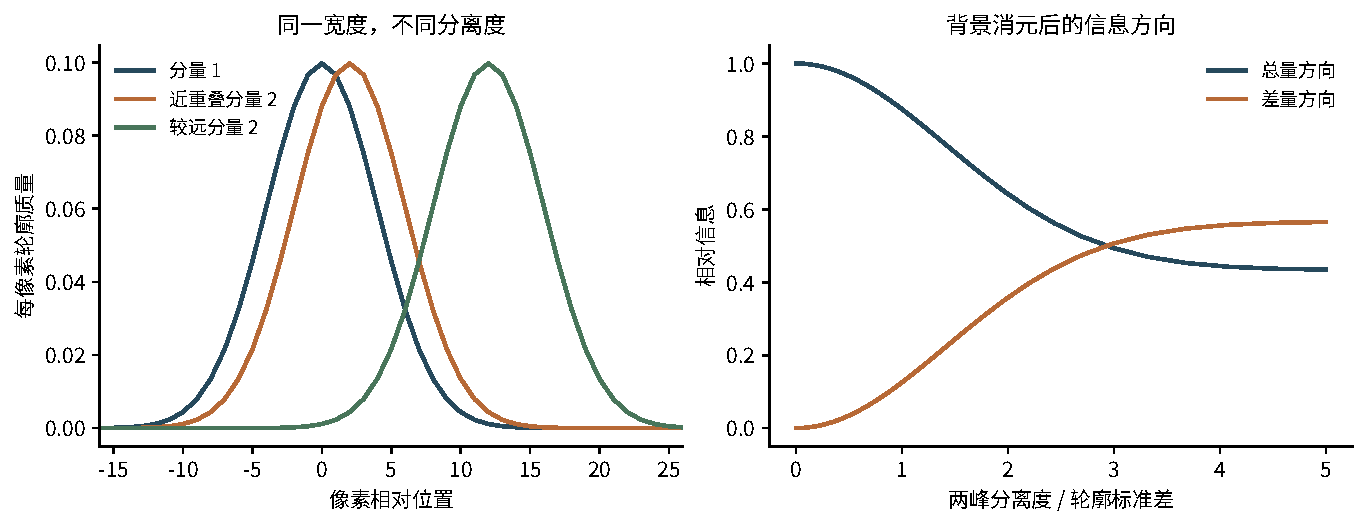
\includegraphics[width=\textwidth]{figures/04_overlap_information.pdf}
\caption{两个高斯轮廓随分离度变化的可辨识性。左侧是轮廓；右侧是背景消元后差量与总量的信息变化。完全重合时差量不可辨识。数据由新压缩接口对固定轮廓计算，所有幅度仍可取正或负。}\label{fig:overlap}
\end{figure}

因此分流依据包括探测器噪声类型、轮廓几何和信息秩。孤立强峰适合校准几何；弱而孤立的峰需要准确背景；严重重叠需要共同像素模型。分流决定如何计算，不决定删去哪些观测。

\section{真实计数与不确定背景}
对已标定的光子计数，
\begin{equation}
 y_i\sim\operatorname{Poisson}(\mu_i),\quad
 \mu_i=(PI+B_g\beta)_i+o_i,\quad I,\beta\ge0.
\end{equation}
这里背景基必须保证非负，$o_i$ 是已知的非负期望计数项。忽略与参数无关的常数，负对数似然为
\begin{equation}
 L=\sum_i[\mu_i-y_i\log\mu_i],\quad
 \nabla_I L=P^{\mathsf T}(1-y/\mu),\quad
 H_I= P^{\mathsf T}\diag(y/\mu^2)P.
\end{equation}
$y_i=0,\mu_i=0$ 的极限要专门处理；$y_i>0,\mu_i=0$ 的似然为无穷差，不能用任意小常数掩盖不可能事件。代码采用稳定的泊松偏差形式，并按行分块计算。

新实现同时拟合背景和信号。对给定的结构预测 $I$，还可调用背景剖面接口求
\begin{equation}
 L_{\rm prof}(I)=\min_{\beta\ge0}L(I,\beta).
\end{equation}
在适用的最优条件下，其一阶导数可以用包络定理直接计算，不需要对每一次背景优化的迭代轨迹求导。

\subsection{用信息尺度计算，避免误判收敛}
优化变量的单位也会影响数值稳定性。代码先按轮廓列和把参数换算到积分计数坐标 $x$，再利用一次优化初值处的期望 Fisher 对角线 $D_j$，令 $s_j=D_j^{-1/2}$、$x_j=s_jt_j$。这样主要方向的局部曲率接近同一量级；在该次优化内保持 $s_j$ 固定，物理似然不变。零曲率方向使用明确的单位尺度回退。

若 $g_j=\partial L/\partial t_j$，非负约束的投影梯度可写为
\begin{equation}
 t_j-\max(0,t_j-g_j)=\min(t_j,g_j),\qquad t_j\ge0.
\end{equation}
两边代数相同，右边更适合浮点计算：左边的大数相减可能把小而非零的分数完全抹掉。新实现用右式的无穷范数判断 KKT 条件，并记录分数所用坐标。

\begin{worked}{检验数值尺度的计数模型}
取单像素 $y=10^{12}$、$\mu=I+10^7$，最大似然解可直接算得 $\widehat I=999990000000$。修复前的大数投影差表达式可能在 $I=10^{12}$ 处误报收敛，其差为十个 $\sqrt y$。本版回归得到 $999990000000.0001$。这是检查浮点判据的代数例子，不是探测器在这一动态范围内可用的实验声明。
\end{worked}

\section{区间为什么不能用一个对称标准差代替}
对感兴趣的组合 $a^{\mathsf T}I=t$，定义
\begin{equation}
 \Delta(t)=2\left[\min_{a^{\mathsf T}I=t,\,I,\beta\ge0}L(I,\beta)-L(\widehat I,\widehat\beta)\right].
\end{equation}
每个试探值都重新拟合背景。常规内部参数可用渐近似然比阈值构造区间；在零边界、低计数或不可辨识情况下，其覆盖率不能直接套用普通高斯理论\cite{chernoff1954}。0.8.0 输出的是带阈值定义的条件剖面区间，并明确记录未做有限样本覆盖率校准。

\begin{worked}{两个像素}
观测为 $(8,3)$，模型为 $(I+b,b)$。最大似然估计是 $\widehat I=5,\widehat b=3$。若将背景当成已知常数，95\% 渐近区间约为 $[0.656,11.892]$；若在每个 $I$ 下重估背景，则约为 $[0,12.419]$。后者较宽，因为数据也需要估计背景。两者差异不是算法精度降低，而是问题中的不确定度被正确保留。
\end{worked}
\begin{figure}[!htbp]
\centering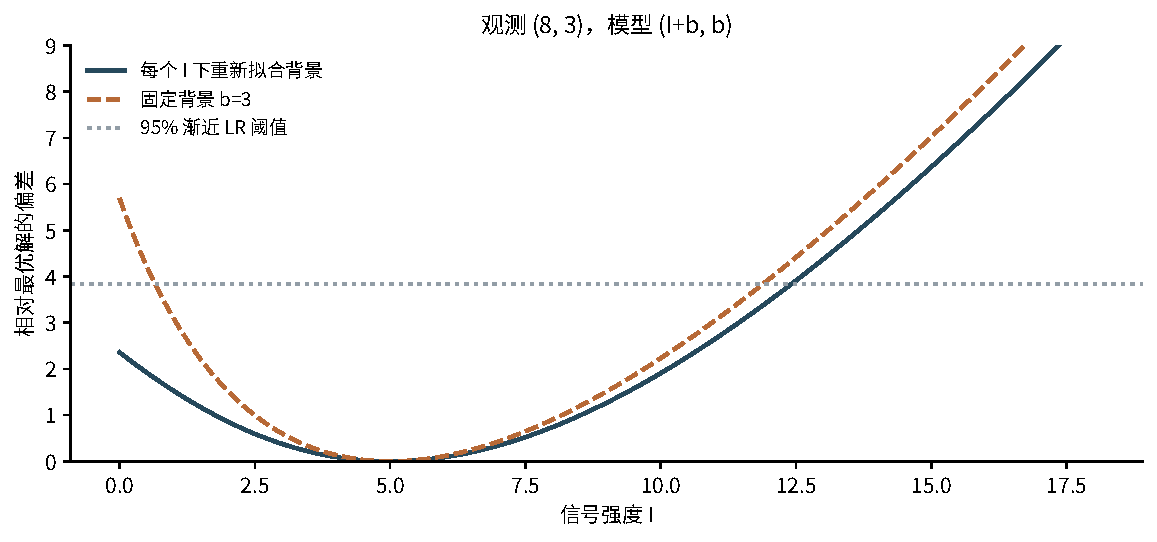
\includegraphics[width=0.95\textwidth]{figures/05_poisson_profile.pdf}
\caption{上述两像素例子的条件剖面偏差。虚线背景固定在 3；实线允许背景重新拟合。水平线采用单参数 95\% 渐近阈值，仅用于展示区间机制。}
\end{figure}

带读出噪声的 ADU 不等于整数光子计数。原有 Ariadne 保留泊松--高斯卷积似然；新分流器检查噪声来源、增益和读出方差声明，卷积后端另要求明确的已去偏置标记。它们不能因为信号弱就自动把 ADU 当成纯泊松计数。

\chapter{尺度、吸收与保留信息的导出}
\label{chap:scaling}

\section{为什么等价反射仍然强弱不同}

理想结构因子只描述晶体内部的相干散射。同一反射在不同扫描位置的观测，
还受入射通量、照射体积、偏振、Lorentz 因子和吸收影响。
若积分结果已经是完整轮廓强度，一个单独反射的前向模型可写成
\begin{equation}
 \operatorname{E}[y_j]=g_jI_{h(j)},\qquad
 g_j=k_j\,L_jP_j\,T_j>0.
 \label{eq:scaling-forward}
\end{equation}
这里 $L_jP_j$ 表示已声明约定的 Lorentz--偏振乘子，并非上一章的体素轮廓矩阵。
实现中的字段是 \code{lp_forward}；方向、单位和是否已经校正必须随数据保存。
完整轮廓积分之后再次除以可见比例，会把同一效应校正两次。

吸收来自光子沿路径的损失。线性吸收系数 $\mu$ 以 mm$^{-1}$ 表示时，
路径长度必须使用 mm。单一路径及有限晶体的平均透过率分别为
\begin{equation}
 T(\bm r)=\exp[-\mu\{L_{\mathrm{in}}(\bm r)+L_{\mathrm{out}}(\bm r)\}],
 \qquad
 \overline T=\frac{1}{V}\int_V T(\bm r)\,d^3\bm r.
 \label{eq:scaling-absorption}
\end{equation}
已知形状与面指数时，这给出物理吸收模型；缺少可靠形状时，多扫描等价反射可以约束经验方向响应。
两者解决的问题相近，但经验系数不应解释成直接测得的晶体形状或绝对吸收系数\cite{scaling2020}。

\section{现有方向模型到底包含什么}

沿用的 Ariadne 全局缩放采用正值指数模型：
\begin{equation}
 g_j=g_j^{\mathrm{known}}\exp(\bm x_j^T\bm\beta).
 \label{eq:scaling-exponential}
\end{equation}
当前代码支持每个扫描的零至二次角度特征，以及关闭吸收项或保留偶二阶方向项。
对共同晶体坐标系中的单位方向 $\bm v=(x,y,z)$，所用基为
\begin{equation}
 H_2(\bm v)=
 (xy,xz,yz,x^2-y^2,3z^2-1)^T,\qquad
 \bm a_j=H_2(\widehat{\bm s}_{\mathrm{in}})
          +H_2(\widehat{\bm s}_{\mathrm{out}}).
 \label{eq:scaling-harmonics}
\end{equation}
这是实二阶球谐空间的一组基，未采用正交归一化常数；系数会吸收该常数。
正值指数保证响应可用作尺度，但经过中心化的相对响应可以大于 1。
它不是必须小于 1 的绝对透过率，也不是任意阶球谐吸收模型。

\section{复合观测应在前向模型中缩放}

重叠组可以给出一个总强度、多个可分辨分量，或一组正交信息模态。
用 $D_b$ 表示这些观测对原贡献的线性映射，$E_b$ 将贡献连接到各自等价反射，则
\begin{equation}
 \bm\mu_b
 =D_b\,\operatorname{diag}\!\bigl(\bm g_b(\bm\beta)\bigr)E_b\bm I.
 \label{eq:scaling-composite}
\end{equation}
单一总量对应一行全 1 的 $D_b$；已辨识分量对应单位阵；压缩 Gaussian 观测则可直接使用上一阶段的 $R$。
这样可以使用不同扫描上的等价信息，而无须先给不可分辨像素强行拆分强度。
每个输入组保留自己的协方差，再统一白化；同一组内的相关分量不能当成互相独立的行。

各孪晶域共享尺度约定也很关键。逐域把平均强度调成一样，会吸收本来属于域体积分数的信息。
保留代码不进行这种独立域归一化；0.8 的结构桥接进一步用结构因子和域分数预测贡献，再进入原观测算子。

\section{尺度规范与变量投影}

强度和尺度存在可交换的乘数：$I\mapsto e^{-c}I$、$g\mapsto e^cg$
不改变预测。现有实现将贡献特征在全局中心化，固定相对尺度规范：
\begin{equation}
 \sum_j\bm x_j=0
 \quad\Longrightarrow\quad
 \sum_j\log\frac{g_j}{g_j^{\mathrm{known}}}=0.
 \label{eq:scaling-gauge}
\end{equation}
这只消除整体规范。若某个方向特征在每个等价反射组内都不变化，它仍可被该组未知强度吸收。
代码另检查组内中心化特征的秩，保留剩余零空间；缺少角度覆盖不会因添加正则项而自动变成实验信息。

给定非线性尺度 $\bm\beta$，有符号强度仍是线性未知量。
把所有白化观测拼成 $\bm d$，相应设计记为 $A(\bm\beta)$，可先求
\begin{equation}
 \widehat{\bm I}(\bm\beta)=A(\bm\beta)^+\bm d,
 \qquad
 \bm r(\bm\beta)=A\widehat{\bm I}-\bm d.
 \label{eq:scaling-varpro}
\end{equation}
这是变量投影\cite{golub1973}。在线性设计保持满列秩的邻域，完整残差导数为
\begin{equation}
 d\bm r=(1-AA^+)(dA)\widehat{\bm I}
          -A^{+T}(dA)^T\bm r.
 \label{eq:scaling-varpro-derivative}
\end{equation}
第二项在残差非零时不能省略。现有实现用 QR/SVD 和固定支撑分组减少重复计算，
避免解正规方程造成条件数平方；满秩条件失效时返回原交替路径，并继续报告秩与收敛证据。
这里的有符号线性解仍然保留负强度估计，不为获得好看的合并统计而截零。

\section{误差传播与导出不能脱节}

设校正后的可测总量为 $S=\bm f^T\bm I$。
如果尺度也从这批强度估计出来，强度与校正因子通常相关，因此
\begin{equation}
 \operatorname{Var}(S)=
 \bm f^TC_I\bm f+\bm I^TC_f\bm I
 +2\bm f^TC_{If}\bm I.
 \label{eq:scaling-cross-covariance}
\end{equation}
最后的同数据交叉项不能因为实现方便而省略。
沿用缩放代码保存联合参数协方差和观测灵敏度，校正阶段据此传播误差。
若像素只给出 $I_1+I_2$，而两分量需要不同的校正因子，仅凭该总量不能得到校正后的和；
应保留复合前向模型，不能用一次结构预测拆分冒充两个新的实验测量。

HKLF 5 是交换格式，不足以装下完整的分量与跨观测协方差。
现有导出器只接受有完整贡献者记录、同相证据和真实校正来源的观测组。
为适应固定小数字段，它可以对所有行共同变换
\begin{equation}
 I'_j=aI_j,\qquad \sigma'_j=a\sigma_j,\qquad a>0,
 \label{eq:scaling-export}
\end{equation}
从而在小数舍入前保持 $I/\sigma$。负强度照常保留；若字段动态范围无法同时容纳有效误差条，
程序保留主数据并报错，不把过小的 sigma 换成任意常数。
非负计数的剖面区间也不能通过“区间宽度除以 2”伪装成 Gaussian sigma。
主 JSON/JSONL 中的似然、协方差和行映射应与 HKL 同时交付。

\begin{table}[!htbp]
 \centering\small
 \caption{沿用的缩放和导出实现；路径前缀为
 \code{skills/ariadne-reduction/scripts/}。}
 \begin{tabularx}{\textwidth}{@{}p{0.40\textwidth}X@{}}
  \toprule
  模块 & 数学对象及作用 \\
  \midrule
  \code{global_scale.py} & \code{harmonics} 与 \code{prepare} 构造共同方向特征、等价关系和观测块。\\
  \code{composite_scaling.py} & \code{fit_global} 联合估计尺度与强度，检查规范、秩与曲率。\\
  \code{variable_projection.py} & 线性强度消元及完整的残差导数。\\
  \code{correct_overlap_groups.py} & 包含同数据交叉项的校正误差传播。\\
  \code{hklf5_stream.py} & 两遍流式格式转换，记录舍入误差与信息损失。\\
  \bottomrule
 \end{tabularx}
\end{table}

本章解释保留的 0.7 数值能力。0.8 新增的是原生像素似然和结构前向桥接，
没有把经验二阶吸收模型重新命名为完整形状吸收，也没有以合成测试代替真实原始帧的缩放验证。

\chapter{相位求解：从直接法到似然双空间迭代}
\section{为什么原子性可以提供相位信息}
已知 $|F_h|$ 而未知 $\phi_h$ 时，可以写出许多密度，但绝大多数不会像由少量原子组成的晶体。直接法利用的正是这种结构限制。对足够分离、形状相近的原子峰，密度平方仍在原来的位置有峰，因此 $\rho^2$ 的傅里叶系数与 $\rho$ 的系数近似具有相同相位。傅里叶卷积定理给出
\begin{equation}
 \mathcal F(\rho^2)_h=\frac1V\sum_k F_kF_{h-k},\qquad
 F_h\simeq C_h\sum_kF_kF_{h-k}.
\end{equation}
这是理解 Sayre 方程的出发点\cite{sayre1952}。它依赖原子形状与分离程度；不能把这种近似当成任意无序、缺失反射或任意组成下都成立的精确测量方程。

不同角度的原子散射因子衰减不同。为减少这一影响，可用组成估计一个平均包络，例如
\begin{equation}
 E_h\approx\frac{F_h}{\sqrt{\sum_j f_j^0(s_h)^2}}.
\end{equation}
实际代码还对包络作整体尺度归一化并设置数值下限。这里得到的是用于搜索的归一化振幅，不是重新标定后的实验强度。

\section{三相位不变量与 tangent 更新}
对于 $h=k+l$，令
\begin{equation}
 \Psi_{hkl}=\phi_h-\phi_k-\phi_l.
\end{equation}
移动原点 $o$ 会使 $\phi_h$ 加上 $2\pi h\cdot o$；由于 $h-k-l=0$，$\Psi$ 不变。这解释了直接法为何可以在未知原点的情况下约束相位。

在经典等原子统计近似下，三相位的浓度随 $|E_hE_kE_l|$ 增大，分布可写成 $p(\Psi)\propto\exp(\kappa\cos\Psi)$。把涉及同一 $h$ 的关系相加，最大化余弦一致性，就得到圆周上的加权平均方向\cite{cochran1955,karle1956}：
\begin{equation}
 \phi_h\leftarrow\arg\sum_{k+l=h}w_{hkl}\exp\{\iu(\phi_k+\phi_l)\}.
\end{equation}
0.8.0 构造有预算的稀疏关系图。权重为归一化振幅乘积再乘各观测的可靠性系数；这是一种搜索引导，不声称是复杂组成下精确的相位后验。阻尼更新为
\begin{equation}
 e^{\iu\phi_h^{\rm new}}\ \parallel\
 (1-\lambda)e^{\iu\phi_h}+\lambda
 \frac{\sum_{k+l=h}w_{hkl}e^{\iu(\phi_k+\phi_l)}}{\sum_{k+l=h}w_{hkl}}.
\end{equation}
如果关系之间互相矛盾，圆均值的模会下降，移动也随之减弱。引导强度在后期衰减，最终不要求观测去满足近似的三相位关系。

\section{双空间法与 intrinsic phasing 的位置}
双空间法交替使用两类约束：倒易空间的振幅或相位关系，实空间的原子峰、稀疏性或密度形状。Shake-and-Bake 是这一思路的重要实现\cite{snb1994}。电荷翻转则把低于阈值的密度改变符号，再回到倒易空间更新\cite{charge2004,charge2008}：
\begin{equation}
 D_\delta(\rho)(x)=
 \begin{cases}\rho(x),&\rho(x)\ge\delta,\\-\rho(x),&\rho(x)<\delta.\end{cases}
\end{equation}
这种更新并非普通凸投影，整个过程通常也没有全局收敛保证，因此需要多起点和独立的结构评价。

SHELXT 的 intrinsic phasing 是一个集成体系：Patterson 与双空间过程在 P1 中产生相位，再处理原点、空间群和元素等问题\cite{shelxt2015}。它不是一条可直接替换所有求解问题的单独公式。Ariadne 借鉴这一分解方式，自行实现相位与原点模块；并不包含 SHELXT 的代码或完整内部策略。

Patterson 函数是密度的自相关：
\begin{equation}
 \mathcal P(u)=\frac1V\sum_h|F_h|^2e^{-2\pi\iu h\cdot u}
 =\int_{\text{cell}}\rho(r)\rho(r+u)\,\dif r.
\end{equation}
它的峰反映原子间向量。新求解器以 Patterson 平移后的最小叠合构造部分起点，其余起点为随机密度。这能利用向量信息，又不把原子真值坐标交给求解器。

\section{弱强度需要柔性的倒易更新}
经典振幅替换把当前复数 $v$ 的模强制设为观测振幅。弱反射的 $\sqrt{\max(y,0)}$ 不适合被当成无误差约束。新实现对每个复系数保留当前相位，只求新的模 $r\ge0$：
\begin{equation}\label{eq:prox}
 r^*=\argmin_{r\ge0}
 \left\{\frac{(r-a)^2}{2\tau}+\frac{(r^2-y)^2}{2\sigma^2}\right\},
 \qquad a=|v|.
\end{equation}
第一项限制本次移动，第二项是带符号强度的高斯似然。$\sigma$ 是强度而非振幅的标准不确定度；$\tau$ 是算法参数，不是探测器测量出的方差。

令 $b=\sigma^2/(2\tau)$，驻点方程成为
\begin{equation}\label{eq:cubic}
 r^3+(b-y)r-ba=0.
\end{equation}
当 $a>0$ 时，存在唯一正根：若 $b-y\ge0$，三次式在正半轴严格递增；若 $b-y<0$，它先下降后上升，而在零点的值已经为负，所以也只有一次向上的穿越。$a=0$ 时直接比较边界和驻点，得到 $r^*=\sqrt{\max(y-b,0)}$。

实现使用按尺度归一化的三次方程、双曲函数和 Cardano 分支，避免为每个反射再启动一个优化器。当 $v\ne0$ 时，更新后的复数为 $r^*v/|v|$；当 $v=0$ 时，径向最优值仍由上式确定，但目标函数不区分相位，代码采用 $\arg(0)=0$ 的确定性约定。低不确定度强度约束较紧，高不确定度强度允许模型形状提供更多搜索方向；负 $y$ 同样参与似然。

若强度单位改变为 $y'=cy,\sigma'=c\sigma$，振幅应变成 $r'=\sqrt c\,r$。为保持算法的尺度协变，代码用工作集的归一化正强度均值设定 $\tau$，使 $\tau'=c\tau$。固定一个与单位无关的 $\tau$ 会破坏这一性质。
\begin{figure}[!htbp]
\centering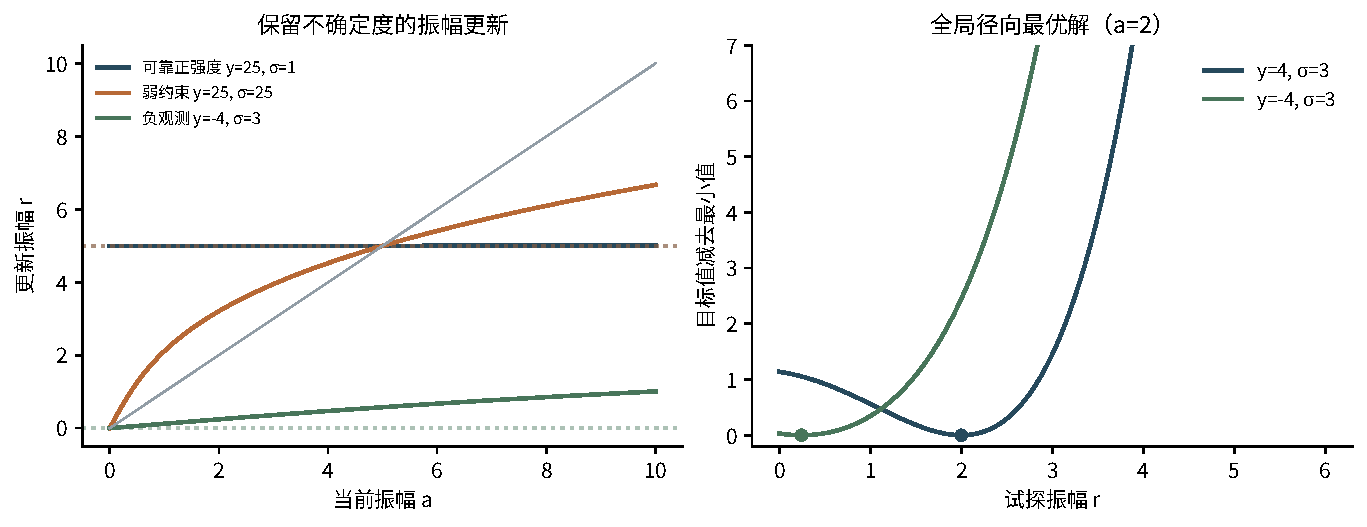
\includegraphics[width=\textwidth]{figures/06_radial_prox.pdf}
\caption{式\eqref{eq:prox}的一维教学示例。横轴是更新前的模，纵轴是求得的模。可靠正强度对目标模约束强；弱正和负强度形成连续、依赖不确定度的更新。虚线是把观测强行转成固定振幅的基线。}
\end{figure}

\section{本版混合求解器的完整循环}
\begin{enumerate}
\item 合并工作集内重复与 Friedel 强度，同时传播方差；验证同一关系轨道没有跨训练和保留角色。实密度求解采用 Friedel 平均，因此不在此步骤推断绝对结构。
\item 按组成建立散射包络、有限三相位图和 FFT 网格。未测到的系数保持为模型变量，不填成“测得的零”。
\item 从随机密度或 Patterson 向量起步；交替作电荷翻转和周期性的有限原子支撑投影。
\item 倒易空间先作衰减的 tangent 引导，再解式\eqref{eq:cubic}。保留 Hermitian 成对关系以及实际倒易度量确定的带宽。
\item 先恢复傅里叶系数的物理散射衰减，再从候选密度提取周期原子峰，用工作强度对候选作初步排序；后续由独立选择集比较精修后的模型。
\end{enumerate}

网格带宽通过倒易度量逐项广播计算，避免同时保存三张完整的整数索引网格。三相位图按候选反射数和每个反射的关系数设上限。多起点仍然是非凸搜索，不能把多跑几轮解释为必定能解。

原有 \code{charge_flip} 与 \code{atomic_projection} 路径保留；新方法名称为 \code{hybrid}。完整晶胞元素数必须由使用者声明。重原子与轻原子混合、分辨率不足、溶剂无序、部分占位和缺失低角反射，都可能削弱原子峰提取。当前实现并未自动推断未知化学式，也未将完全混合的孪晶总强度直接当成一个晶畴的 $|F|^2$。

\chapter{原点、空间群与模型约束}
\section{对称关系必须同时作用于相位}
设分数坐标对称操作为 $x\mapsto Rx+t$。保持晶体密度不变意味着
\begin{equation}
 F(hR)=\exp(-2\pi\iu h\cdot t)F(h),
\end{equation}
此处 $h$ 采用代码中的行向量记号。若 P1 候选相对于标准设置还差一个原点平移 $o$，其结构因子会乘上 $e^{2\pi\iu h\cdot o}$，于是应检验
\begin{equation}\label{eq:sg-phase}
 F(hR)\exp\{2\pi\iu[h\cdot t+(hR-h)\cdot o]\}-F(h)=0.
\end{equation}
这个公式同时解释了三件事：空间群判断需要相位；原点有时必须搜索；纯平移导致的消光不能通过移动原点消除。

\section{搜索的是候选假设}
新模块对显式给出的候选空间群做度量兼容性检查，然后最小化式\eqref{eq:sg-phase}的归一化复残差。原点的 Jacobian 直接来自指数函数：
\begin{equation}
 \frac{\partial r_{h,o}}{\partial o_j}
 =2\pi\iu(hR-h)_jF(hR)
 e^{2\pi\iu[h\cdot t+(hR-h)\cdot o]}.
\end{equation}
有限网格和由原子对得到的起点共同初始化局部优化。若 $hR-h$ 只张成二维空间，那么第三个原点方向没有被该群的相位关系固定；程序报告这个秩，而不假装找到了唯一原点。

P1 的相位不一致度恒为零，因此不能简单把所有群按这个数排序，再宣布最小值就是正确空间群。低不一致度只允许产生一个新的结构候选。最终还需要看系统消光、等价反射一致性、几何投影和独立选择数据。

\section{从 P1 全晶胞到非对称单元}
原点对齐之后，每个对称操作应把一组原子映到同元素的另一组原子。代码使用周期晶胞度量计算距离，并通过一对一分配避免多个原子同时认领同一个位置。若操作后的最大匹配距离超过声明的容差，该候选被拒绝。

将一个对称轨道内匹配的原子逆变换回代表位置，可得若干坐标估计：
\begin{equation}
 x_{jo}^{\rm back}=R_o^{-1}(x_{\pi_o(j)}+n_{jo}-t_o).
\end{equation}
整数平移 $n_{jo}$ 用最小周期距离确定，平均后得到对称化位置。位移张量也必须作相同的逆旋转。完成投影后，再展开全部物理位置，核对元素数、占有率和坐标偏差。

对斜晶胞，直接把每个分数坐标差四舍五入未必得到最近的晶格平移。保留的 \code{Cell.minimum_image} 用三维球形分支限界求最近晶格向量，供配对、几何限制和验证统一使用。

\begin{worked}{任意原点下的反演结构}
将一个斜晶胞中的 $P\overline1$ 六原子全晶胞任意平移后，用原点搜索和对称投影可以恢复三个原子的非对称单元。本次独立测试的相位不一致度约为 $1.95\times10^{-30}$，含原点相位因子后的结构因子差小于 $5.3\times10^{-14}$。这是恒等关系与实现一致性的检查，不是未知实验数据空间群识别率。
\end{worked}

\section{精确约束与柔性限制}
空间群规定的特殊位置是精确约束。例如反演中心上的坐标不应靠一个很强的弹簧“拉近”，而应从自由变量中消去。用 $x=x_0+Tv$ 表示允许的坐标切空间，可避免无意义的自由度和奇异法方程。

键长、键角、平面性通常属于模型知识的柔性限制。例如
\begin{equation}
 L_{\rm bond}=\frac12\left(\frac{d_{ij}(\theta)-d_0}{\sigma_d}\right)^2.
\end{equation}
$\sigma_d$ 控制允许偏离的程度。理想 MOF 的连接关系可以帮助选择 $d_0$，但它仍是先验知识。最终报告应分开给出衍射残差和限制残差，并检查某个参数是否主要由限制而不是数据确定。

\chapter{精修：直接求导并消除无效自由度}
\section{目标函数与物理参数}
对已校正、可视为独立的带符号强度，原生精修最小化
\begin{equation}
 Q(\theta)=\sum_{h\in\mathcal W}w_h[y_h-I_h(\theta)]^2
             +\sum_m r_m(\theta)^2.
\end{equation}
第一项使用工作集，第二项是明确给出的结构限制。$w_h=1/\sigma_h^2$ 是基本选择。保留的经验权重模式使用外层冻结权重迭代；每次最小二乘只对这一轮固定的权重求导，并记录权重是否达到固定点。训练使用全部有效 $F^2$，$I>2\sigma(I)$ 只出现在传统 $R_1$ 指标的定义里\cite{shelxl2015}。

\section{解析导数的来源}
令原子某一对称位置的贡献为 $C_{joh}$。对任意独立实参数 $p$，
\begin{align}
 \partial_p C_{joh}
 &=C_{joh}\left(2\pi\iu h^{\mathsf T}\partial_p x_{jo}
      -2\pi^2q^{\mathsf T}(\partial_pU_{jo})q\right)
      +\text{占有率的贡献},\\
 \partial_p|F_h|^2&=2\operatorname{Re}(F_h^*\partial_pF_h).
\end{align}
占有率为零时，不能用 $C/o_j$ 这种形式求导；应直接保留不含占有率的原子贡献。新实现按这一点处理边界。强度尺度 $k$、晶畴比例和对称操作的导数再用链式法则组合。

原实现对每个参数作两次扰动，再重算整张衍射表。新实现只计算一遍当前原子贡献，再累积所有非零切向导数。原子散射因子、固定倒易几何和位置轨道提前缓存；反射按块计算，减少同时存放的复数数组。

\section{正定位移参数与矩阵指数}
各向同性位移参数写为 $u=e^v$，其导数为 $\dif u=u\dif v$。一般位置的各向异性张量用 Cholesky 形式：
\begin{equation}
 U=LL^{\mathsf T},\qquad L_{ii}=e^{v_i},\qquad
 \dif U=(\dif L)L^{\mathsf T}+L(\dif L)^{\mathsf T}.
\end{equation}
这样每次迭代都满足正定性，而不是先得到负特征值再裁切。

特殊位置还要求 $U$ 位于对称性不变的子空间。代码在相应的对称矩阵空间中写 $U=\exp S$。若 $S=Q\diag(s_i)Q^{\mathsf T}$，矩阵指数的 Fréchet 导数为
\begin{equation}
 D\exp(S)[E]=Q\left[K\odot(Q^{\mathsf T}EQ)\right]Q^{\mathsf T},\qquad
 K_{ij}=\begin{cases}
 \dfrac{e^{s_i}-e^{s_j}}{s_i-s_j},&s_i\ne s_j,\\e^{s_i},&s_i=s_j.
 \end{cases}
\end{equation}
重复特征值并不使导数不存在。数值上用 $e^{(s_i+s_j)/2}\operatorname{sinhc}[(s_i-s_j)/2]$ 求这个连续商，避免对不稳定的特征向量进行差分。

\section{比例约束与尺度规范}
晶畴比例和一组和固定的占有率可以用 softmax 表示，固定参考 logit 为零：
\begin{equation}
 \alpha_d=\frac{e^{v_d}}{\sum_ce^{v_c}},\qquad
 \frac{\partial\alpha_d}{\partial v_c}=\alpha_d(\delta_{dc}-\alpha_c).
\end{equation}
固定参考值消除了所有 logit 同时加常数的冗余。它仍不能消除物理模型本身的退化。例如把所有占有率乘 $c$、把强度尺度除以 $c^2$，可能保留相同的计算强度。因此至少需要一个占有率锚点或精确的组成和约束。

P1 中整体平移原子坐标也不改变强度。连续原点自由度应通过明确的规范消去。空间群中的特殊位置多重度是离散选择，不能在连续优化末尾悄然改变；新代码检查这种变化，要求重新声明位置模型。

\section{不通过大矩阵估计信息}
残差的线性化为 $r(\theta+\delta)\approx r+J\delta$。若 $J$ 有零空间，沿相应方向改变参数不会一阶改变观测。代码不再构造完整的观测维左奇异矩阵，而是按块累积
\begin{equation}
 R_{t+1}=\operatorname{qr}_R\begin{bmatrix}R_t\\J_{t+1}\end{bmatrix},
 \qquad R=U_R\Sigma V^{\mathsf T}.
\end{equation}
正交变换保留奇异值，所以可用小矩阵的 $\Sigma,V$ 判断参数秩。条件协方差只在可辨识且处于常规内部的参数上有通常解释：
\begin{equation}
 C_\theta=V\Sigma^{-2}V^{\mathsf T},\qquad
 C_p=G C_\theta G^{\mathsf T},\quad G=\partial p/\partial\theta.
\end{equation}
秩不足时返回零空间和可估计子空间的伪逆；不把伪逆的对角线当作不可辨识参数的真实标准差。受边界影响的标准差同样标明适用范围。报告还分别给出仅由衍射提供的秩和加入限制后的秩。

新的复杂临时数组按反射块大小增长；当前 SciPy 信赖域求解器仍保存实数 $N\times p$ Jacobian，所以不能说整个精修过程只用常数内存。下一步可以在同一导数接口上实现矩阵自由的 $Jv$、$J^{\mathsf T}v$ 和迭代线性求解；本版没有把这项计划写成已实现功能。
\begin{figure}[!htbp]
\centering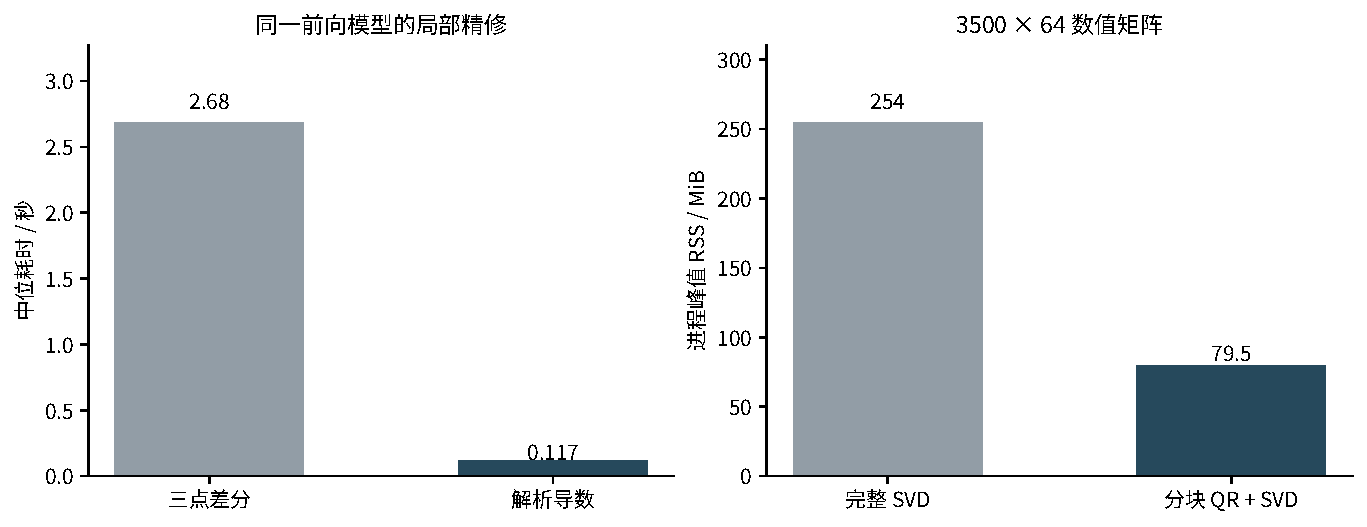
\includegraphics[width=\textwidth]{figures/07_refinement_performance.pdf}
\caption{本次环境中的局部数值基准。左：18 原子、1,098 反射、70 参数的三次单线程中位时间；两条路径使用同一缓存前向模型。右：3500\,$\times$\,64 矩阵的独立进程峰值 RSS，包含解释器和库开销。它们不是与 SHELXL 的速度比较。}\label{fig:performance}
\end{figure}

\chapter{让结构直接解释重叠像素}
\section{用一个共同结构连接多个区域}
逐个重叠点去孪晶，要求每一组像素独立确定所有分量。这个要求有时过强，因为各个反射来自同一个原子结构。可以先保留第三章的观测似然，再把结构预测代入：
\begin{equation}\label{eq:joint-residual}
 r_g(\theta,\alpha)=R_g\diag(c_g\alpha_{d_g})\,k|F_{h_g}(\theta)|^2-z_g.
\end{equation}
联合目标是
\begin{equation}
 Q(\theta,\alpha)=\sum_{g\in\mathcal W}\bigl[\|r_g\|^2+c_g^{\rm residual}\bigr]
                  +Q_{\rm restraints}(\theta).
\end{equation}
这里的 $c_g$ 是各分量校正系数向量，$c_g^{\rm residual}$ 是压缩残差常数，两者不要混淆。每个分量有独立的 Miller 指数和所属晶畴编号。多个晶畴共享一个结构的前提是它们属于同一相，接口要求显式声明这一点。

对于背景已按线性高斯模型消元的像素，这个目标与在原始像素上逐次重估背景的目标相同。精修没有把相关估计变成独立行，也没有先求一张唯一的去孪晶强度表。

\section{解析导数如何穿过观测算子}
令 $v_g(\theta)=k|F_{h_g}(\theta)|^2$。结构参数和晶畴比例的 Jacobian 分别为
\begin{align}
 \partial_\theta r_g&=R_g\diag(c_g\alpha_{d_g})\,\partial_\theta v_g,\\
 \partial_u r_g&=R_g\diag(c_gv_g)\,\partial_u\alpha_{d_g}.
\end{align}
前一章的衍射导数可以直接复用；第二式使用 softmax 的导数。整个结构精修看到的是小型 $R_g$，不用重复加载大量高斯像素。若轮廓、掩膜、方差或背景基发生变化，必须重新压缩；旧 $R,z$ 不能跨越这种模型变化继续当作同一个似然。

\section{局部不可分与全局不可辨识不同}
一个区域只有 $I_1+I_2$ 的信息，并不意味着全部结构参数都不可辨识。若许多区域的 $h_1,h_2$ 不同，它们对原子坐标的导数也不同，堆叠后的结构 Jacobian 可能满秩。此时确定的是“共同结构模型下的参数”，并不是每个区域突然多出了一次独立测量。

本次三原子合成例中，171 个区域都可以设为完全重叠，每个局部信号矩阵均为秩 1；共享结构后仍得到 11 个可辨识参数，恢复给定的 $(0.73,0.27)$ 晶畴比例。这是局部已知模型附近的计算实验，说明这种机制可行；它不证明完全重叠的未知结构总能从头求解。

\begin{figure}[!htbp]
\centering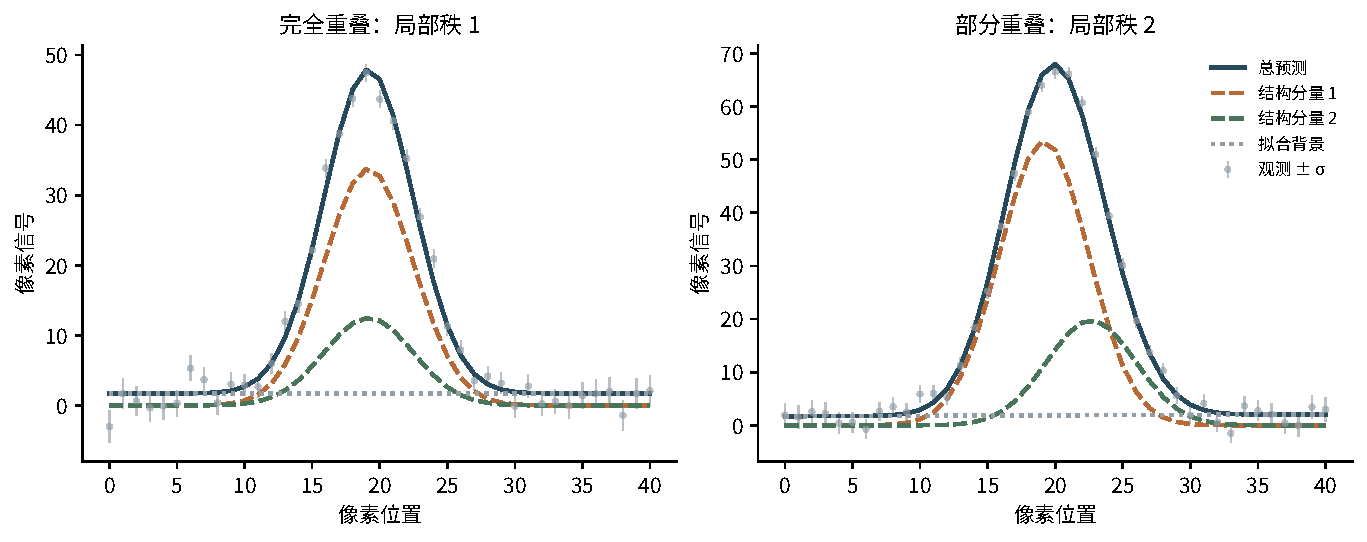
\includegraphics[width=\textwidth]{figures/08_joint_pixels.pdf}
\caption{联合精修的两个合成区域。观测像素只与总预测比较；彩色分量曲线是共享结构给出的解释，并非独立测量。一个区域完全重叠，另一个部分重叠。绘图数据来自本次 7,011 像素的含噪声精修结果。}
\end{figure}

\section{一个必须失败的反例}
若两个晶畴仅互为反演，且没有反常散射，实电子密度满足 $F_{-h}=F_h^*$。于是
\begin{equation}
 \alpha|F_h|^2+(1-\alpha)|F_{-h}|^2=|F_h|^2,
 \qquad\frac{\partial\mu_h}{\partial\alpha}=0.
\end{equation}
任何精修算法都无法从这些数据确定 $\alpha$。优化器可能在平坦方向停在某个值，甚至靠近 0 或 1，但这个值没有测量意义。新接口分别保存内部数值代表和可报告的参数估计；上述情形中比例估计为 \code{null}，并给出秩不足的方向。

这也是闭环的关键约束：结构知识可以缩小一类解释，不能凭空补出实验从未区分过的信息。若必须借助化学先验确定某一方向，应报告先验条件下的结果及其敏感性。

\section{强、弱与复杂孪晶的统一路线}
几何隔离清楚的反射适合提供相位初始化。全部有效区域随后进入共同结构似然，包含弱峰和严重重叠区域。前者负责“找到一个合理起点”，后者负责“检验并改进这个起点”。一批数据在初始化和最后精修中都被使用并不自动造成重复计数；只要最终目标中每份观测只出现一次，初值本身不是第二份测量。

如果没有足够的隔离反射，原生从头求解应明确停止这一分支，要求已有结构假设或其他可验证的相位来源。对混合相、调制结构、显著漫散射或需要动力学散射的情况，也不能继续套用同相运动学模型。

纯计数像素目前由联合泊松信号--背景模块处理，并能对给定结构强度剖面背景。自动的压缩观测求解与 \code{joint-refine} 使用固定方差高斯路径；完整的泊松像素结构优化、几何和吸收联合精修属于下一阶段工程，不能用高斯压缩接口偷偷代替。

\chapter{原生智能体与结构反馈闭环}\label{ch:loop}
\section{闭环应该更新什么}
完整问题可以写成一个联合模型：
\begin{equation}
 p(\theta,\alpha,\eta,\beta\mid y,M)
 \propto p(y\mid\theta,\alpha,\eta,\beta)\,
 p(\theta\mid M)p(\alpha)p(\eta)p(\beta).
\end{equation}
$M$ 表示组成、化学连接或候选结构类型。观测 $y$ 固定；闭环更新的是对结构、几何、背景或晶畴的解释。结构因子预测应进入前向模型或作为明确的先验，不能替换原始像素后再把替换结果当作另一份实验。

0.8.0 的可执行实现分成两层。数值层提供有物理定义的求解器、导数、似然和诊断；智能体层规定下一步计算、数据角色、预算和输出。宿主大模型可以提出一个有类型的操作请求，软件只执行注册过的算子。模型生成的文字不会被当作晶体测量，也不会直接作为 Python 或 shell 代码运行。

\section{三种数据角色}
将独立证据分为 $\mathcal W$、$\mathcal S$、$\mathcal A$，分别用于拟合、选择和审计。对第 $m$ 个候选：
\begin{equation}
 \widehat\theta_m=\argmin_\theta L_{\mathcal W}(\theta;M_m),\qquad
 m^*=\argmin_m L_{\mathcal S}(\widehat\theta_m;M_m).
\end{equation}
选定候选后可以用 $\mathcal W\cup\mathcal S$ 再精修一次，随后只评价一次 $\mathcal A$。审计结果写入最终报告，不据此再自动调参。这是本版控制器实际执行的顺序。

不能随意逐行随机分割。等价反射、Friedel 对、同一个像素组的多个分量以及显式声明的共享测量应处于同一个连通分量。代码以 Miller 关系和重叠连接生成图，再按连通分量分配角色；不以观测符号或信噪比选择数据。已有的预留标记会被保留，若标记切开同一证据分量则报错。

这仍然是给定预处理模型下的验证。若仪器几何、轮廓或吸收已经利用了所有数据，强度层的保留集不能宣称整个原始图像处理也完全独立。严格的实验比较还应在外层按扫描块或独立采集划分，并重新执行相应标定。

\begin{figure}[!htbp]
\centering
\begin{tikzpicture}[>=Latex,node distance=8mm and 11mm,
 box/.style={draw=ink!50,fill=pale,rounded corners=2pt,align=center,text width=35mm,minimum height=12mm,font=\small}]
\node[box] (e) {关联证据分组\\等价、Friedel、共像素};
\node[box,below left=of e] (w) {work\\生成与拟合};
\node[box,below=of e] (s) {selection\\选择候选};
\node[box,below right=of e] (a) {audit\\封存};
\node[box,below=18mm of s] (m) {唯一选定模型\\可用 work+selection 再拟合};
\node[box,below=of m] (f) {最终报告\\一次独立评价};
\draw[->] (e)--(w);\draw[->] (e)--(s);\draw[->] (e)--(a);
\draw[->] (w)--node[above,font=\scriptsize]{候选}(s);
\draw[->] (s)--(m);\draw[->] (m)--(f);
\draw[->,accent,thick] (a.east)--++(7mm,0)|-(f.east);
\draw[->,ink!55] (s.south west)--++(-6mm,-8mm)-|(w.south);
\end{tikzpicture}
\caption{控制器的数据职责。候选之间可以在工作与选择证据上比较；审计分支只有通向最终评价的路径。改变审计数据的数值不应改变已经选择的结构。}
\end{figure}

\section{从隔离反射启动，再使用全部区域}
新的 \code{solve-observations} 流程以压缩高斯像素组为输入。初始化时只选几何上隔离、属于参考晶畴的单分量组，不按强度阈值筛选。若该组的压缩矩阵是一列 $r$，则它给出
\begin{equation}
 \widehat I=\frac{r^{\mathsf T}z}{r^{\mathsf T}r},\qquad
 \sigma_I^2=\frac1{r^{\mathsf T}r}.
\end{equation}
已知分量系数需同时作用于估计和标准不确定度。参考晶畴的全局比例只改变初始强度尺度，不应改变相位搜索；新版的尺度协变更新正是为此设计的。

这些带符号初始观测只负责生成模型。每个模型随后在全部 work 像素组的共同似然上精修，包括弱点、部分重叠和完全重叠。选择分支比较同一批 selection 组。不可辨识的单点分量不需要先分拆，也不会被导出成一张虚构的独立强度表。

输入已经有合理模型时，控制器可以跳过从头相位阶段，执行同一套分组、联合精修、模型选择和审计。没有模型、也没有足够的隔离相位数据时，当前实现会清楚报告缺少可用的初始化证据。这比从任意孪晶总强度构造一个未经物理证明的振幅集合更可检查。

\section{MOF 的理想结构能提供什么}
已知金属节点、配体、化学计量或拓扑，可以明显减少模型空间。例如已知配体的键长角度约束、刚性片段、对称性候选，都可以降低弱数据下的参数方差。一个常见的数学形式是
\begin{equation}
 Q_\lambda(\theta)=\chi^2_{\rm diffraction}(\theta)
                  +\lambda\|g(\theta)-g_0\|_{\Sigma_g^{-1}}^2.
\end{equation}
$g_0$ 来自独立化学知识，$\lambda$ 表示对它的信任程度。数据弱时先验的作用更大，因此结论也更依赖先验。应比较合理的备选模型，例如完整节点与缺陷节点、不同客体占有率、合理的无序形式，而不是只允许朝一个理想结构移动。

当前原生内核已提供距离、角度、相似距离、平面性、ADP 相似和刚性键等限制，以及精确的占有率和位置约束。它没有内置一个经过全面验证的 MOF 拓扑生成器，也不会自动把化学上“看起来顺眼”的原子补成实验已经观察到的原子。理想模型的可信部分用于提出候选，衍射似然负责检验候选。

\section{何时回到上游}
残差的形状可以提示下一个可检验的问题。反射位置随转角系统漂移，提示检查几何；峰两侧残差符号相反，提示质心或宽度；一个区域出现与第二晶格一致的额外峰，提示新的晶畴假设；残差随入射／出射方向变化，提示吸收模型。每次只修改相关前向假设，并保存前后模型。

本版保留的 DIALS 工作流与新的 \code{native.run} 算子可放入同一个持久化有向图。进程具有时间、重试、日志和取消预算；每次尝试保留独立目录、输入快照和结果。重启后可以继续已存在任务，而不是丢掉前面的证据重算。

原生控制器目前自动执行的是明确的候选搜索、局部精修和验证规则。根据所有残差自主重新标定仪器、发现任意混合相、重建未知 MOF 化学的完整闭环，还需要专门的假设生成器与实验标定。接口已经能表达这些分支，但不能把一个工具调用框架写成全部科学决策都已经实现。

\section{判断闭环是否有价值}
对固定审计集，比较新旧流程的预测似然、误差条覆盖、结构偏差和资源消耗。训练残差下降只说明优化器更擅长拟合训练数据。若新增结构先验降低训练误差、却恶化审计似然，控制器应保留这一失败证据。

本次集成测试还做了一个直接检查：将封存审计数据的强度和不确定度极端改变，候选生成、候选选择及最终拟合模型仍应完全不变，只有审计指标改变。这个测试检验的是计算路径是否泄漏，并不替代跨样品的科学验证。

一次最终评价由每次原生求解流程控制。传输失败后以相同输入、请求和随机种子重算，是计算恢复；看到审计结果后更换假设或调参，是新的模型选择。后者需要新的外层评价设计。任务哈希和断点恢复能保证计算来源，不能使已经公开的审计数据重新变得独立。

\chapter{让数学决定 C++ 内核的边界}\label{chap:kernels}

\section{先找真正重复的计算}
精修每走一步，都要重新计算许多反射的结构因子及其导数。坐标约束、特殊位置、晶畴比例和统计目标决定\textbf{算什么}；对每个反射、每个原子位置重复执行的乘加、指数和三角函数决定\textbf{怎样高效地算}。本版把后者实现为可选的 C++17 内核，保留前者在可检查的 Python 模型中。已有的 FFT、BLAS 和 SciPy 线性代数继续使用其现成实现。

选择这一边界有实际剖析依据。在三原子、三晶畴、7,280 个反射的 NumPy 路径中，12 次不同参数的预测调用有约 $88.2\%$ 的剖析时间位于结构因子块计算。主要开销来自复数数组、张量收缩及其临时结果。剖析用于定位；本章的速度比使用另行计时的运行结果，避免把剖析器开销计入加速收益。

\section{由复数微分直接得到实数 Jacobian}
固定一个反射，令第 $s$ 个对称位置\textbf{不含占有率}的贡献为
\begin{equation}
 C_s=(f_s+f_s'+\iu f_s'')
      \exp[-2\pi^2q^{\mathsf T}U_s q]
      \exp[2\pi\iu h^{\mathsf T}x_s],
 \qquad F=\sum_s o_s C_s .
\end{equation}
对独立实参数 $p$，定义
\begin{equation}
 \gamma_{sp}=-2\pi^2q^{\mathsf T}(\partial_pU_s)q,
 \qquad \phi_{sp}=2\pi h^{\mathsf T}\partial_px_s .
\end{equation}
则
\begin{equation}
 \partial_p F=\sum_s C_s
   \left[\partial_po_s+o_s\gamma_{sp}+\iu o_s\phi_{sp}\right].
\end{equation}
写 $F=u+\iu v$、$C_s=a_s+\iu b_s$，把
$\partial_p|F|^2=2\operatorname{Re}(F^*\partial_pF)$ 展开，得到
\begin{equation}\label{eq:fused-kernel-jacobian}
 \boxed{\partial_p|F|^2=
 \sum_s \left\{
 2(ua_s+vb_s)(\partial_po_s+o_s\gamma_{sp})
 +2(va_s-ub_s)o_s\phi_{sp}\right\}.}
\end{equation}
这个式子只需要实数累加。计算顺序是先求一个反射的 $F$，暂存这个反射各位置的 $a_s,b_s$，再把各位置的非零参数切向直接累加到一行实数 Jacobian。占有率导数保留 $\partial_po_s$，因此 $o_s=0$ 时仍然有定义。

NumPy 参考实现先形成一块 $B\times P$ 的复数 $\partial F/\partial p$，再与 $F^*$ 相乘并取实部。融合内核省去了这个复数矩阵及相应复数收缩临时量。内核循环的额外暂存为 $O(S+P)$：$S$ 是展开后的原子位置数，$P$ 是独立参数数；打包的稀疏切向另占 $O(S+T)$，其中 $T$ 是非零位置--参数关联数。每块仍需输出实数 $B\times P$ 导数。

晶畴与强度尺度的链式法则同样可以避免大数组复制：
\begin{equation}
 I=k\sum_d\alpha_d I_d,\qquad
 \partial_pI=k\sum_d\left(\alpha_d\partial_p I_d+
          I_d\partial_p\alpha_d\right)
        +\left(\sum_d\alpha_d I_d\right)\partial_pk .
\end{equation}
代码把域贡献直接累加到最终 Jacobian 的块视图；比例和尺度的导数只更新其非零参数列。这个改动同时改善两种后端，消除了原来只为广播少数尺度参数而分配的整块矩阵。

\begin{principle}
本版降低的是结构因子计算的临时存储。SciPy 精修仍保存完整实数 $N\times P$ Jacobian；已经存在的几何和散射因子缓存也保留。融合内核没有把整个精修变成常数内存算法。
\end{principle}

\section{弱反射要求认真处理相消}
弱反射有时是多个较大原子贡献相消的结果。即使各项计算准确，依次相加也可能把较小项舍去。内核对 $F$ 的实部、虚部以及导数累积采用补偿求和。以一项 $a$ 加入当前和 $s$ 为例，Neumaier 更新为
\begin{align}
 t&=s+a,\\
 c&\leftarrow c+
 \begin{cases}
 (s-t)+a,&|s|\ge |a|,\\
 (a-t)+s,&|s|<|a|,
 \end{cases}\qquad s\leftarrow t .
\end{align}
最后使用 $s+c$。这里 $c$ 收集普通加法丢失的低位。代码保持固定的位置累积顺序，编译时关闭 fast-math 和浮点乘加收缩，避免编译器重新结合这些有意安排的运算。

一个独立的数值压力检查采用零相位项
$10^{16},1,-10^{16},1$。80 位十进制参考给出 $F=2$、$|F|^2=4$；当前环境的普通 NumPy 求和得到 $F=1$，补偿内核得到正确的 $|F|^2=4$，共同占有率方向的导数为 $8$。这是检查浮点求和的人工例子。物理检查则使用 $P2_12_12_1$ 晶体，与 Gemmi 独立结构因子计算器比较：三个系统消光反射的计算强度均低于 $4.45\times10^{-27}$，允许反射也满足设定的数值容差。

补偿求和改善的是舍入误差。相位三角函数的误差、像素计数噪声和结构模型不确定性仍由各自的数值精度与统计模型处理。弱反射的置信区间沿用前文的观测似然；编译内核不增加观测信息。

\section{接口、线程与可重复性}
绑定只依赖 CPython 的缓冲区接口，不依赖 NumPy C 头文件、pybind11 或特定的复数二进制布局。输入使用本机字节序的 \code{float64} 与有符号 \code{int64}；复数在 C++ 中以两个实数表示。Python 包装层为非连续或未对齐的视图准备合适的块缓冲区。C++ 入口检查类型、维数、形状与字节数、对齐、整数范围、有限值以及输出别名；空反射块在分配暂存前返回。每个已取得的缓冲区通过局部对象自动释放\cite{python-buffer}。

进入数值循环后释放 GIL，循环结束再恢复；释放期间不调用 Python API\cite{python-threads}。该内核始终只有一个线程，不启动 OpenMP。外层 agent 调度负责并行运行独立动作，并为已有的数值库设置每个动作的线程预算。输入数组在一次调用期间应保持不变；不同任务可同时调用各自的预测器。

运行后端与构建选择相互独立：
\begin{center}
\begin{tabularx}{\textwidth}{lX}
\toprule
选择 & 行为\\
\midrule
\code{ARIADNE_BUILD_CPP=auto} & 安装时尝试可选编译；编译失败仍可安装 Python 功能。\\
\code{ARIADNE_BUILD_CPP=0} & 构建纯 Python 包。\\
\code{ARIADNE_BUILD_CPP=1} & 要求编译成功；失败使构建失败。\\
\code{ARIADNE_NUMERIC_BACKEND=auto} & 扩展可导入时使用 C++，否则使用 NumPy 并记录原因。\\
\code{ARIADNE_NUMERIC_BACKEND=python} & 明确使用 NumPy 参考实现。\\
\code{ARIADNE_NUMERIC_BACKEND=cpp} & 要求 C++；扩展不可用时明确报错。\\
\bottomrule
\end{tabularx}
\end{center}

已有 Python 依赖、C++17 编译器及当前 Python 头文件时，可在 \code{native/} 目录复现：
\begin{lstlisting}
python tools/build_optional_kernel.py --inplace
python -m ariadne_xtal.kernels
OPENBLAS_NUM_THREADS=1 python validation/run_v08_kernels.py
python validation/check_v08_kernel_build.py
\end{lstlisting}
状态接口报告实际后端、编译器、架构和线程策略；普通精修及观测组精修结果也记录后端。运行中的数值错误不会触发另一套实现的静默重算。构建检查实际验证了纯 Python wheel、编译 wheel 的独立目录导入，并用不可用编译器检查了可选构建与强制构建的不同行为。

\section{实际收益与适用范围}
本次验证平台为 Linux x86\_64、CPython 3.12.14、GCC 13.3.0；NumPy、SciPy、Gemmi 分别为 2.3.5、1.17.0、0.7.5。BLAS 线程固定为 1。两种后端使用相同物理模型、解析导数、起始参数和收敛设置。预测器测试每轮连续计算八组不同参数，重复五轮取中位数；表中的预测时间已除以八。完整局部精修重复三轮。

\begin{center}
\begin{tabular}{lrrr}
\toprule
计时范围 & NumPy / ms & C++ / ms & 速度比\\
\midrule
三原子、三域，$N=7280,P=17$ & 28.77 & 7.86 & 3.66\\
32 原子、单域，$N=4096,P=126$ & 44.74 & 14.55 & 3.08\\
18 原子完整局部精修，$N=1098,P=70$ & 113.50 & 61.42 & 1.85\\
\bottomrule
\end{tabular}
\end{center}

前两项包含参数解包、对称位置准备、全部晶畴的强度和 Jacobian，并非单独一个 C++ 函数的理想吞吐率。第三项还包含优化器、秩分析和协方差，因此加速幅度较小。它保留 18 个负观测强度；两个后端精修后的预测差异为 $4.52\times10^{-11}$ 倍标准差的均方根，两种预测案例的最大按列尺度归一化导数差异低于 $1.90\times10^{-14}$。

内存测试在各自独立的进程中计算同一个 80 原子、8,192 反射、318 参数问题。块长 $B=1024$ 时，总峰值 RSS 从 $103.3$ 降为 $93.0$ MiB；$B=8192$ 时从 $168.0$ 降为 $110.5$ MiB。RSS 包含解释器、库、输入、缓存和输出，不等同于纯临时数组大小。返回的完整实数 Jacobian 本身约占 $19.9$ MiB。较小反射块已经限制了 NumPy 的临时内存，所以 C++ 的总内存优势会随块大小变化。

\begin{figure}[!htbp]
\centering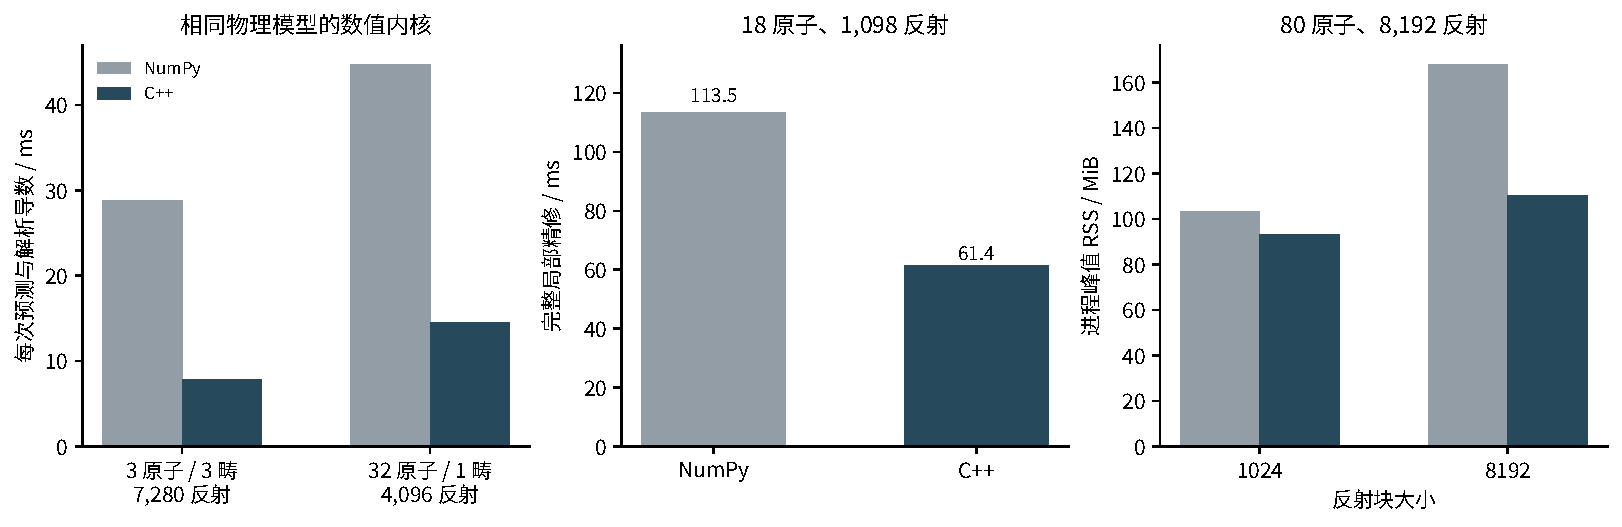
\includegraphics[width=\textwidth]{figures/10_cpp_kernel.pdf}
\caption{可选 C++ 内核的局部实测。左：两种规模的强度及解析 Jacobian，每种后端五轮、每轮八次计算，中位轮时间除以八。中：18 原子完整局部精修的三轮中位时间。右：相同输入的独立进程总峰值 RSS，分别使用两种块长。完整测量及源码摘要保存在 \code{v08_kernel_measurements.json}。}\label{fig:cpp-kernel}
\end{figure}

这组结果支持在重复的结构因子累积处使用融合内核。完整数据还原、FFT 相位检索及任意大型结构的收益需要按各自负载衡量；本章的数值对应明确给出的合成预测问题和已知附近起点的局部精修。发行包同时提供可移植的纯 Python wheel、C++17 源码，以及本平台实编译验证的 CPython 3.12 Linux x86\_64 wheel。

\chapter{有资源预算的智能体任务调度}
\label{chap:scheduler}

\section{把计算组织成有向无环图}
一次结构解析通常包含多个候选：不同相位初值、空间群、晶畴模型或原子指派。它们能够共享输入，但不一定相互依赖。用有向无环图 $G=(V,E)$ 表示计算，节点 $v$ 是一次有明确输入和输出的动作，边 $u\to v$ 表示 $v$ 必须读取 $u$ 的结果。普通节点的就绪条件是
\begin{equation}
v\in\mathcal R\quad\Longleftrightarrow\quad
v\text{ 尚未执行，且 }\operatorname{pred}(v)\text{ 全部成功完成}.
\end{equation}
任务图因此同时说明了\textbf{哪些计算可以并行}和\textbf{结果从哪里来}。模型建议执行一个动作，调度器仍会检查它是否就绪、引用是否属于声明的依赖、输入文件是否与保存的哈希一致。

\begin{figure}[!htbp]
\centering
\begin{tikzpicture}[node distance=9mm and 13mm,>=Latex,
 box/.style={draw=ink!50,fill=pale,rounded corners=2pt,text width=39mm,minimum height=10mm,align=center,font=\small}]
\node[box] (inputs) {冻结的输入快照};
\node[box,below left=of inputs] (a) {候选 A 的原生精修};
\node[box,below right=of inputs] (b) {候选 B 的原生精修};
\node[box,below=27mm of inputs] (review) {汇集结果及失败证据};
\node[box,below=of review] (package) {校验并打包产物};
\draw[->] (inputs)--(a);\draw[->] (inputs)--(b);
\draw[->] (a)--(review);\draw[->] (b)--(review);
\draw[->] (review)--(package);
\end{tikzpicture}
\caption{双起点精修的依赖关系。输入在会话初始化时保存；两个精修动作独立执行，汇总节点等待二者结束。汇总成功表示证据已汇集，并不自动宣布某个结构成立。}
\end{figure}

\section{资源约束是明确的加法}
令正在执行的节点集合为 $\mathcal A$，节点申请的线程数和内存额度分别为 $c_v,m_v$。调度器只在以下条件同时成立时接纳一个新任务：
\begin{equation}
|\mathcal A|\le W,\qquad
\sum_{v\in\mathcal A}c_v\le C,\qquad
\sum_{v\in\mathcal A}m_v\le M.
\label{eq:resource-admission}
\end{equation}
其中 $W$ 是工作进程数上限，$C$ 是总线程额度。只有设置了总内存额度 $M$，才应用第三项。单个任务申请超过总额度会在执行前被拒绝，避免任务永远处于就绪却无法启动的状态。

这里的 $m_v$ 是用户声明的\textbf{准入额度}，不是已经测量的常驻内存，也不是操作系统强制上限。大量反射、密集 Jacobian 或大 FFT 网格应申报较大的额度；调度器不会根据原子数猜测一个精确内存值。CPU 额度传给 OpenMP、OpenBLAS、MKL 等合作线程库；它不限制任意外部程序自行派生的进程数。当前注册的外部适配器另有自己的参数契约。

\begin{longtable}{p{0.30\textwidth}p{0.20\textwidth}p{0.41\textwidth}}
\toprule 配置项 & 默认值 & 含义\\\midrule
\code{max_workers} & 1 & 同时执行的动作数上限。\\
\code{cpu_threads} & 等于工作数 & 全会话的线程额度。\\
\code{memory_mb} & \code{null} & 总声明内存额度；空值表示不按内存准入。\\
\code{default_task_memory_mb} & 256 & 节点未声明时使用的额度。\\
\code{isolate_actions} & 工作数大于 1 时为真 & 是否为每个动作启动独立解释器；并发时必须为真。\\
节点 \code{resources} & 1 线程、默认内存 & 可按动作覆盖 \code{cpu_threads} 和 \code{memory_mb}。\\
\bottomrule
\end{longtable}

增加工作数只利用现有的独立性。若各动作所需时间为 $t_v$，关键依赖链的总时间为 $L$，在每个动作使用一个执行槽的简化模型中，总墙钟时间至少为
\begin{equation}
T\ge\max\left(L,\frac{\sum_v t_v}{W}\right).
\end{equation}
启动解释器、读取数据和内存带宽竞争还会增加实际时间。因此，大量短动作不一定因并发而变快。输出同时记录实际墙钟时间和 \code{cumulative_action_seconds}；后者是各动作持续时间之和，在并发时可以大于墙钟时间，不能当作测得的 CPU 时间。

\section{计算进程、决策线程与提交者}
默认单工作模式保留原有顺序行为。启用隔离后，每个动作通过新的 Python 解释器启动，拥有独立的进程组、日志和 \code{attempts/node/attempt} 目录，路径分别标识节点和尝试号。这里采用 \code{subprocess}，避免在已有决策线程的进程中直接 \code{fork} 出计算进程\cite{python-process}。NumPy 等库导入前便获得线程环境；原生 C++ 内核在内部采用单线程，外层候选任务可以由调度器并行。

计算进程写自己的产物和完成记录，父调度进程负责接纳结果、更新节点状态、传播失败和扩展任务图。外部适配器可以记录本次子进程 PID，但不能自行增加下游节点。每个进程使用独立 SQLite 连接，完成提交使用事务。模型决策在单独的线程中处理一个只读快照；返回建议后，父进程重新检查当前依赖和额度。取消后到达的建议会被丢弃，不再启动计算。

\section{失败、取消和恢复}
普通依赖失败后，下游尚未执行的节点标记为 \code{skipped}，并保留原因。专门的汇总节点可以声明接受失败依赖，从而把成功产物和失败日志一起交付；它不会伪造缺失的科学结果。

隔离动作的子进程继承本动作的进程组。取消或超时时，父进程先请求退出，再杀死未退出的成员，并回收直接子进程。每个工作进程还监视一条仅由父调度器持有写端的管道：父进程崩溃或被 \code{SIGKILL} 终止时，管道关闭，工作进程终止自己的整个进程组。该机制覆盖本包的 \code{native.run} 嵌套调用链；外部程序若自行脱离进程组成为守护进程，需要专门的适配器。

同一会话由操作系统文件锁保护，只允许一个 runner 修改执行状态。输入快照、节点定义和成功产物在再次运行时校验；已完成节点直接复用。崩溃时若数据库仍记为 \code{running}，程序不会假定动作未执行，也不会自动重放。确认旧进程已结束后，\code{recover} 将该次尝试记为中断；需要重算时再显式 \code{retry}。完成结果可检查、失败过程可解释，状态与文件不会混成一个“成功”字符串。

\code{cancel} 请求停止；\code{resume} 只清除取消标记。\code{run --steps N} 最多接纳 $N$ 个动作，然后等待已启动动作结束。预算按会话累计，分次运行不会重新获得已用的动作数或时间。活动 runner 用单调时钟计时；跨进程状态显示和崩溃恢复使用持久化时间戳，恢复值保守地包括未确认的停机间隔。

进程监督与文件锁支持 Linux、macOS 和 WSL，本次进程树验证在 Linux 上完成。Windows 原生环境可以导入模块，但该持久化执行器明确要求 POSIX 环境。若单工作任务也需要在阻塞计算中被强制取消，应设置 \code{isolate_actions=true}；默认进程内的 Python 动作只能在检查点发现超时。

\section{并行候选仍需独立的科学验证}
任务隔离解决的是计算与产物的边界。统计独立性仍由第\ref{ch:loop}章的数据划分保证：工作集用于产生和拟合候选，选择集比较候选，冻结的审计集在最后评价。多个候选可以同时拟合同一工作集，这不会增加独立观测数；把同一审计集反复用于调整策略，则会改变它的统计角色。

同一冻结请求、输入和随机种子的数值动作，因进程或传输故障而重算，不等于利用审计结果调参。改变物理假设、候选策略或验证划分时，应建立明确的新实验记录。调度器本身不会把重复执行包装成新证据，也不会替代数值 API 内部的选择和审计规则。

\section{可复现的实际运行}
\code{examples/v08/parallel_native.json} 对公开 FeN$_4$ 的 71 个实测强度，从两个给定起点并行调用原生精修，再汇集结果和打包\cite{fen4}。第二个起点对两个 N 原子施加小坐标扰动，并将其各向同性位移参数乘以 1.2；Fe 的反演中心位置不变。这是已知模型再精修，不是从头相位成功率试验。

\begin{lstlisting}
ariadne-agent init examples/v08/parallel_native.json runs/parallel-demo
ariadne-agent run runs/parallel-demo
ariadne-agent status runs/parallel-demo
python benchmarks/v08_scheduler.py --with-tests
\end{lstlisting}

实际时间线见图\ref{fig:scheduler-timeline}。完整记录写在
\code{docs/v08/results/scheduler_validation.json}，包括测试命令、数量、运行平台、峰值资源额度、事件时间线，以及两个原生精修结果文件的哈希。测试覆盖真实原生子进程的并发、依赖、内存和线程准入、动态扩图、启动失败、取消、超时、父进程崩溃、同会话锁及恢复；外部 SHELX 动态扩图测试采用明确标注的协议夹具。

本次定向回归的 86 项测试全部通过，其中新增调度测试 17 项。实际双起点流程的峰值为两个工作进程、两个 CPU 额度和 512 MB 声明内存额度；总墙钟时间为 1.825 秒，动作持续时间之和为 2.546 秒。两个起点均收敛到 $R_1(\mathrm{all})=0.0412682$、$wR_2=0.0814805$，再次运行未重做任何已完成动作。此处时间用于核对并发和依赖行为，没有作为一般加速比使用。

\begin{figure}[!htbp]
\centering
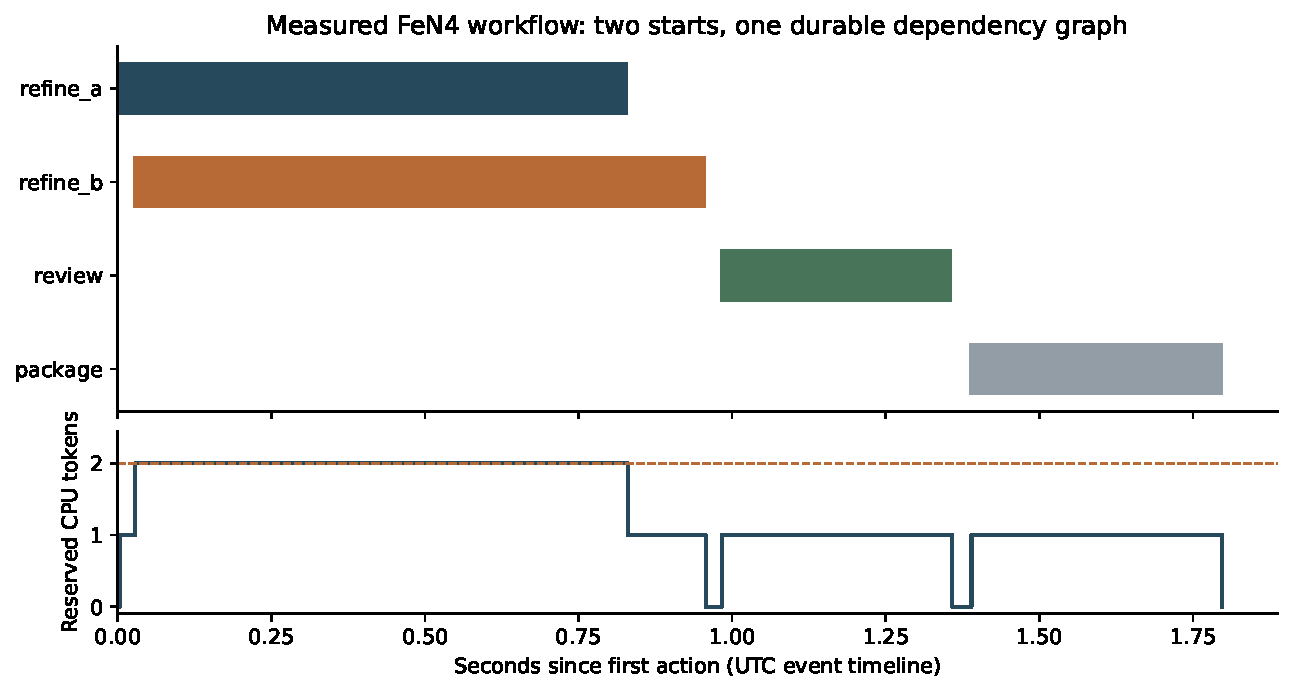
\includegraphics[width=0.96\textwidth]{figures/14_scheduler_timeline.pdf}
\caption{实际 FeN$_4$ 双起点工作流的调度时间线。色条包含解释器启动、计算和结果提交；两个精修动作同时存在，review 与 package 遵守依赖顺序。下图显示保留的 CPU 额度，不是操作系统测得的 CPU 利用率。时间线取自事件时间戳，执行预算使用单调时钟。}
\label{fig:scheduler-timeline}
\end{figure}

\chapter{软件组织与可替代的工作范围}
\label{chap:software}
\section{一个项目，两套可独立安装的内核}
代码包保留原 Ariadne 的 Python 包、DIALS 源码补丁、数据还原脚本和持久化 agent，加入原生 \code{ariadne-xtal} 子包。原生结构计算不要求安装 SHELXT/SHELXL；DIALS 原始图像处理需要单独的 DIALS/cctbx/dxtbx 环境。

\begin{longtable}{p{0.32\textwidth}p{0.60\textwidth}}
\toprule 目录或入口 & 职责\\\midrule
\code{python/src/ariadne/} & 持久化工作流、旧能力与新像素似然；\code{reduction_native.py} 为新增可导入数值接口。\\
\code{native/src/ariadne_xtal/} & 相位、对称、结构因子、解析精修、重叠结构拟合和原生自动求解。\\
\code{skills/ariadne-reduction/} & 保留的原始帧处理方法、几何／体素／全局缩放／导出脚本。\\
\code{patches/} & 针对指定 DIALS 基线的源码补丁；不是已编译的 DIALS 安装。\\
\code{tests/}, \code{tests_rebuild/} & 数据还原、agent、反馈、工具契约和本次新像素接口的测试。\\
\code{native/tests/} & 散射、相位、对称、精修、传输和新闭环测试。\\
\code{native/validation/} & 合成盲解、已知结构再精修、性能和联合观测的复现脚本、结果。\\
\code{docs/v08/} & 本书、独立 loop 报告、图与 LaTeX 源文件。\\
\bottomrule
\end{longtable}

\section{安装与最小运行}
在代码包根目录，使用 Python 3.12 创建新环境。避免把旧环境的包目录直接混入新环境；数值库应安装成一套完整版本。
\begin{lstlisting}
python3.12 -m venv .venv
. .venv/bin/activate
python -m pip install --upgrade pip
python -m pip install -e './python[dev]' -e './native[dev]'
ariadne-xtal capabilities
ariadne-xtal run examples/v08/autosolve.json --root examples/v08
\end{lstlisting}
源码包内的示例生成脚本先产生带标签的合成数据；实际运行及输出目录见中文指南。低依赖路径只需要 NumPy、SciPy、Gemmi；图形展示另需 Matplotlib、Plotly 和 scikit-image，完整安装文件已声明这些依赖。

结构输入支持原生 JSON、小分子 CIF 与结构性 INS/RES 导入；反射 JSON 保留精度与验证标记，传统 HKLF4 用于兼容交接。CIF/RES 的结构导出不等于执行其全部 SHELXL 精修指令。官方后端桥接仍然保留，但必须显式指定已有可执行文件，不会静默替代原生求解器。

\section{给 agent 的操作语言}
\begin{longtable}{p{0.25\textwidth}p{0.67\textwidth}}
\toprule 操作 & 输入与输出的科学含义\\\midrule
\code{integrate} & 给定像素、轮廓、背景基和噪声标定，生成高斯观测似然或联合计数拟合。没有仪器信息时不猜增益。\\
\code{solve} & 已知晶胞与完整晶胞元素表，生成 P1 相位候选；不自动接受结构。\\
\code{autosolve} & 独立强度表上的原生相位、候选精修、可选空间群投影与三角色验证。\\
\code{symmetry} & 显式空间群列表上的原点相位检验和非对称单元投影。\\
\code{refine} & 带符号 $F^2$、约束／限制、各向异性参数和适用的面网孪晶精修。\\
\code{joint-refine} & 压缩像素组直接约束同相结构和晶畴比例。\\
\code{solve-observations} & 从隔离组初始化，使用全部 work 组联合精修，选择后评价一次 audit。\\
\code{maps}, \code{absolute} & 密度、Patterson、残差图，以及声明模型下的绝对结构诊断。\\
\code{native.run} & 在原 Ariadne 持久化 agent 中以受预算约束的子进程执行上述操作。\\
\bottomrule
\end{longtable}

JSON 请求中的文件路径只能引用所选工作区内的输入。输出保存为新的运行目录，包含请求、环境、输入快照、结果和图。原生 JSONL 与 MCP 都调用同一个数值分派器；主 agent 还支持任务图、超时、恢复和失败证据。

\section{相对于旧代码的实质变化}
直接法、Patterson、QR、变量投影和矩阵指数都已有成熟数学来源。本次新增的价值在于将这些原理形成可执行的组合，并修复具体的信息损失和计算浪费，不把经典恒等式重新命名为原创理论。

\begin{longtable}{p{0.27\textwidth}p{0.31\textwidth}p{0.32\textwidth}}
\toprule 问题 & 原有路径 & 本次实现\\\midrule
弱反射相位约束 & 主要为固定振幅的电荷翻转 & 带符号强度近端更新，尺度协变、三相位阻尼与原子支撑交替。\\
空间群衔接 & 消光与等价关系诊断 & 增加原点相位搜索、一对一原子轨道配对和精确 ASU 投影。\\
精修导数 & 每个参数三点差分 & 缓存、分块的解析衍射 Jacobian，包含特殊位置、ADP 与比例约束。\\
不确定度内存 & 完整左奇异向量矩阵 & 分块 QR 加小矩阵 SVD，保留秩与零空间。\\
重叠与结构衔接 & 像素拟合后交接强度 & 将保留的观测算子直接作用于 $|F(\theta)|^2$，可共同估计同相畴比例。\\
计数背景 & 原有计数模型与边界工具 & 新可导入接口共同估计背景，剖面区间重估背景，并给结构预测返回解析分数。\\
自动闭环 & 独立工具与持久任务图 & 原生从头／初模流程，连通证据分组，候选选择与一次最终审计。\\
\bottomrule
\end{longtable}

\section{与 SHELXT/SHELXL 工作的对应关系}
\begin{longtable}{p{0.31\textwidth}p{0.60\textwidth}}
\toprule 任务 & 0.8.0 原生状态\\\midrule
从头相位求解 & 已实现已知组成、P1 起步的多起点混合求解；已有小规模合成盲解。\\
空间群、原点 & 显式候选群检验和投影已实现；未覆盖 SHELXT 全部自动 Laue 群、元素分配与未知组成策略。\\
基本结构精修 & 坐标、尺度、各向同性／各向异性位移、占有率和约束已实现。\\
孪晶 & 原生支持面网比例精修；压缩像素接口支持有明确索引和轮廓的同相多晶畴共同精修。不是任意 HKLF5 指令流的完整解析器。\\
无序与化学限制 & 提供原生约束和限制；完整 AFIX/HFIX、自动骑乘氢、FRAG 和全部自由变量语言尚未实现。\\
绝对结构 & 保留显式反常散射、反演比例及 Friedel 商诊断；无信息时报告不可辨识。\\
高级校正与报告 & 原还原侧的缩放／吸收与导出保留；完整消光、溶剂掩膜、中子散射及正式 checkCIF 全流程尚未替代。\\
原始帧处理 & 保留 DIALS 适配与源码补丁。本次没有用户原始衍射帧，也没有在此环境执行原生 DIALS 全流程。\\
\bottomrule
\end{longtable}

独立数值内核已经成立，成为一套独立的软件路线是合理的；是否足以替代某个实验室的生产流程，需要用该实验室的样品、仪器和交付标准验证。源码中保留官方后端适配，是为了让尚未覆盖的工作仍能继续，而非把外部结果混入原生算法成绩。

\chapter{怎样验证这套实现}
\label{chap:validation}
\section{先检验数学身份，再检验求解能力}
软件会输出一个数字，不代表这个数字正确。本次验证分为四层：基础恒等关系和独立导数检查；受控合成数据恢复；公开实验强度的已知模型再精修；真实命令行与持久化 agent 的集成执行。它们回答不同问题，结果分别保存。

衍射导数使用另一路物理计算及中心差分检查，覆盖斜晶胞、反常散射、非对称平移群、特殊位置重根 ADP、占有率和约束以及多个孪晶畴。径向近端更新用独立的三次方程驻点计算检查全局最优；相位算法还检验原点协变、强度单位协变、Friedel 配对和保留集不泄漏。

像素压缩对任意结构预测与原始像素直接剖面比较，而不只在拟合最优点比较。这样可以确认后续结构搜索在整个可检查区域内看到同一个目标。共同像素结构精修同时检查恢复例和必然不可辨识的反演反例。

\section{从头求解的受控实验}
所有相位实验只提供晶胞、观测、不确定度和完整晶胞元素表，不提供真值原子坐标。恢复误差在允许原点、反演和同元素置换后计算。真值只用于产生数据和事后评价。

\begin{table}[tb]
\centering\small
\caption{本次合成盲解。每个场景四个起点全部得到可精修模型；表中 RMS 为代表结果，不能外推成实验成功率。}
\begin{tabularx}{\textwidth}{@{}Xrrr@{}}
\toprule 场景 & 观测数 & 负强度数 & 精修后 RMS / $\angstrom$\\\midrule
四碳，第一噪声档 & 4540 & 397 & 0.00106\\
四碳，第二噪声档 & 4540 & 868 & 0.00254\\
四碳，第三噪声档 & 4540 & 1298 & 0.00843\\
斜晶胞 O$_2$N$_2$C$_4$ & 4590 & 125 & 0.000997\\
\bottomrule
\end{tabularx}
\end{table}

四碳例使用四次起点、每次 400 轮，混合元素例为四次起点、每次 600 轮。结果说明带符号弱强度可以参与此求解机制；它们不是高无序 MOF、大晶胞或未知组成的验证集。

独立强度表的自动流程将 4540 条观测按关联分为 work 3406、selection 680、audit 454。四个起点产生候选后，选择并再精修一个模型；审计标准化残差 RMS 为 0.9653，坐标 RMS 为 $0.000979\angstrom$。该审计指标没有用于挑选起点。

\section{从混合观测组开始的自动流程}
合成双畴例有 2497 个高斯观测组，包括隔离、近重叠和完全重叠。work、selection、audit 分别为 1861、381、255 组。只用 work 中 1121 个隔离参考畴观测初始化相位，其中有 95 个负强度；它们仍然保留。

四个相位起点经过共同结构精修后均收敛。选择模型的晶畴比例约为 $(0.63237,0.36763)$，合成真值为 $(0.63,0.37)$；坐标 RMS 为 $0.002203\angstrom$，一次最终审计的模式标准化 RMS 为 1.02375。整个过程使用观测算子，没有把无法分离的分量当成独立测量。这是压缩高斯证据上的集成盲解，尚不是仪器原始帧重处理实验。
\begin{figure}[!htbp]
\centering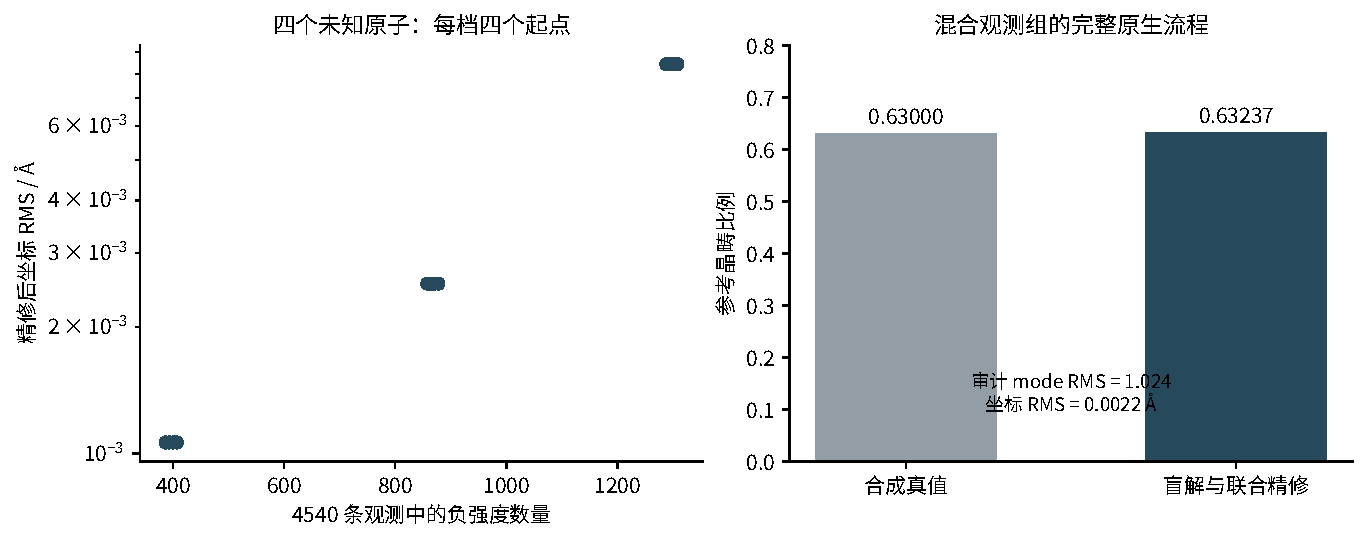
\includegraphics[width=\textwidth]{figures/09_blind_recovery.pdf}
\caption{左：三种噪声条件下的四起点盲解。横坐标仅描述数据，不用于裁掉负值。右：双畴混合观测流程恢复的比例与设定真值。数据来源为本次 \code{v08_phasing/result.json}。}
\end{figure}

\section{局部结构精修与不确定度}
对于 171 个区域、7011 个像素的三原子局部精修例，混合重叠和全部完全重叠两种设计都恢复了设定结构与 $(0.73,0.27)$ 的比例。全部重叠时，各区域信号秩为 1，但共享结构的 Jacobian 为 11/11。含噪声时参考畴比例为 0.7301858，条件标准不确定度为 0.0006302，最大坐标误差约 $0.003365\angstrom$。

最终 C++ 路径上，同一含噪数据的压缩目标与原像素背景剖面目标之差为 $-9.09\times10^{-13}$。若改成无反常散射的反演孪晶，结构 Jacobian 为 10/11，软件返回不可辨识的比例估计与空协方差。一个正确的求解器既要能恢复有信息的参数，也要识别没有信息的参数。

\section{实验数据回归：\texorpdfstring{FeN$_4$}{FeN4}}
公开数据来自 Bykov 等人的 FeN$_4$ 单晶研究及所存测量强度\cite{fen4}。本次读取 71 个实测 $F^2$ 与标准不确定度，从公开模型和一个扰动后的模型分别开始，使用原生散射和精修器；没有把文件中的计算结构因子当作观测，也没有调用 SHELXL 数值后端。

\begin{table}[tb]
\centering
\caption{FeN$_4$ 已知模型的实验强度再精修。此表验证一个给定模型的数值一致性，不评价从头求解。}
\begin{tabular}{@{}lrr@{}}
\toprule 指标 & 本次原生计算 & 公开参考值\\\midrule
$R_1\,[I>2\sigma(I)]$ & 0.040316 & 0.0403\\
$R_1$，全部观测 & 0.041268 & 0.0413\\
$wR_2$ & 0.081480 & 0.0815\\
拟合优度 & 1.183324 & 1.183\\
独立参数数 & 10 & 10\\
\bottomrule
\end{tabular}
\end{table}

使用的是同一个特定权重模型、各向同性位移参数和明确的特殊位置约束。良好一致性为原生内核提供实验数据支持，但一个样品不代表全部元素、消光、无序和孪晶功能已经等价。

\section{效率的测量范围}
\begin{table}[tb]
\centering\small
\begin{tabularx}{\textwidth}{@{}Xrr@{}}
\toprule 本机测量 & 基线 & 新路径\\\midrule
18 原子、1098 反射、70 参数精修中位时间 & 2.6817 s & 0.11729 s\\
同一精修的衍射前向调用数 & 988 & 7\\
3500\,$\times$\,64 SVD 例进程峰值 RSS & 260500 KiB & 81444 KiB\\
25 万像素增广 QR 的额外峰值分配 & 43.82 MB & 0.516 MB\\
该像素例的一次测量耗时 & 0.0215 s & 0.0595 s\\
\bottomrule
\end{tabularx}
\end{table}

精修时间比较明确使用同一 NumPy 缓存前向计算，区别是差分与解析导数；在本例中约快 22.9 倍，最终预测差在 $10^{-9}\sigma$ RMS 以下。C++ 与 NumPy 的同一解析模型比较另见第\ref{chap:kernels}章，不能把不同计时口径直接相乘。像素例比较的是预分配输入以外的额外分配，基线仅作稠密 QR，新路径还完成背景消元及信息分解。新路径在这一例中更省工作内存，但更慢；不能把内存比写成时间加速比。

记录环境为 Python 3.12.14、NumPy 2.3.5、SciPy 1.17.0、Gemmi 0.7.5。精修时间取三次单线程中位数；内存进程和像素分配实验各有明确口径，JSON 中保留原始数值。

\section{复现和下一批实验}
冻结源码后的完整回归包含 572 项通过的主测试，以及 136 个通过的子测试。还原侧为 366 项通过、11 项跳过；原生结构侧为 206 项通过、没有跳过，并启用了真实 MCP 标准输入输出测试。11 个跳过项需要当前环境没有安装的 DIALS、cctbx 或 dxtbx。C++ 数值测试和新增调度测试已经计入这些总数，不能重复相加。

完整相位、共同观测精修和 FeN$_4$ 回归又以明确指定的 C++ 后端生成了最终数值记录；前述差分与解析导数性能比较则明确指定 NumPy 后端。编译 wheel 与纯 Python wheel 另在独立目录检查实际导入和运行，使编译扩展缺失时的行为也有执行证据。

\begin{lstlisting}
python -m pytest tests tests_rebuild -q
ARIADNE_MCP_STDIO_TEST=1 python -m pytest native/tests -q
python benchmarks/v08_reduction.py
python native/validation/run_v08_refinement.py
python native/validation/run_v08_kernels.py
python native/validation/run_v08_joint.py
python native/validation/run_v08_phasing_autonomy.py
python native/validation/run_real_fen4.py
python docs/v08/tools/make_figures.py
\end{lstlisting}
测试应在两个独立 pytest 进程中运行，避免旧测试目录中同名模块和互相导入造成收集冲突。DIALS 相关测试只在具备真实原生运行环境时执行；本包的测试记录明确列出跳过项，不将它们计为通过。最终汇总见随包验证文件。

接下来最有价值的数据不是再增加一个容易的合成例，而是固定一批真实 MOF 原始帧：包括常规强衍射、不同弱信号比例、部分与完全重叠、溶剂无序和已知缺陷。应预先固定判断标准、外层扫描块划分和计算预算，比较反射预测残差、积分覆盖率、共同观测预测似然、结构误差和总运行资源。只有这些实验才能回答生产替代的范围。

\backmatter
\begin{thebibliography}{99}
\small\linespread{1.0}\selectfont\setlength{\itemsep}{2pt}\setlength{\parskip}{0pt}
\bibitem{dials2018} Winter G, Waterman D G, Parkhurst J M, et al. DIALS: implementation and evaluation of a new integration package. Acta Crystallographica D, 2018, 74: 85--97. \href{https://doi.org/10.1107/S2059798317017235}{doi:10.1107/S2059798317017235}.
\bibitem{scaling2020} Beilsten-Edmands J, Winter G, Gildea R, et al. Scaling diffraction data in the DIALS software package: algorithms and new approaches for multi-crystal scaling. Acta Crystallographica D, 2020, 76: 385--399. \href{https://doi.org/10.1107/S2059798320003198}{doi:10.1107/S2059798320003198}.
\bibitem{sayre1952} Sayre D. The squaring method: a new method for phase determination. Acta Crystallographica, 1952, 5: 60--65. \href{https://doi.org/10.1107/S0365110X52000137}{doi:10.1107/S0365110X52000137}.
\bibitem{cochran1955} Cochran W. Relations between the phases of structure factors. Acta Crystallographica, 1955, 8: 473--478. \href{https://doi.org/10.1107/S0365110X55001485}{doi:10.1107/S0365110X55001485}.
\bibitem{karle1956} Karle J, Hauptman H. A theory of phase determination for the four types of non-centrosymmetric space groups $1P222$, $2P22$, $3P_12$, $3P_22$. Acta Crystallographica, 1956, 9: 635--651. \href{https://doi.org/10.1107/S0365110X56001741}{doi:10.1107/S0365110X56001741}.
\bibitem{snb1994} Miller R, Gallo S M, Khalak H G, Weeks C M. SnB: crystal structure determination via shake-and-bake. Journal of Applied Crystallography, 1994, 27: 613--621. \href{https://doi.org/10.1107/S0021889894000191}{doi:10.1107/S0021889894000191}.
\bibitem{charge2004} Oszlányi G, {\latintext Sütő} A. Ab initio structure solution by charge flipping. Acta Crystallographica A, 2004, 60: 134--141. \href{https://doi.org/10.1107/S0108767303027569}{doi:10.1107/S0108767303027569}.
\bibitem{charge2008} Oszlányi G, {\latintext Sütő} A. The charge flipping algorithm. Acta Crystallographica A, 2008, 64: 123--134. \href{https://doi.org/10.1107/S0108767307046028}{doi:10.1107/S0108767307046028}.
\bibitem{shelxt2015} Sheldrick G M. SHELXT -- Integrated space-group and crystal-structure determination. Acta Crystallographica A, 2015, 71: 3--8. \href{https://doi.org/10.1107/S2053273314026370}{doi:10.1107/S2053273314026370}.
\bibitem{shelxl2015} Sheldrick G M. Crystal structure refinement with SHELXL. Acta Crystallographica C, 2015, 71: 3--8. \href{https://doi.org/10.1107/S2053229614024218}{doi:10.1107/S2053229614024218}.
\bibitem{french1978} French S, Wilson K. On the treatment of negative intensity observations. Acta Crystallographica A, 1978, 34: 517--525. \href{https://doi.org/10.1107/S0567739478001114}{doi:10.1107/S0567739478001114}.
\bibitem{golub1973} Golub G H, Pereyra V. The differentiation of pseudo-inverses and nonlinear least squares problems whose variables separate. SIAM Journal on Numerical Analysis, 1973, 10: 413--432. \href{https://doi.org/10.1137/0710036}{doi:10.1137/0710036}.
\bibitem{chernoff1954} Chernoff H. On the distribution of the likelihood ratio. Annals of Mathematical Statistics, 1954, 25: 573--578. \href{https://doi.org/10.1214/aoms/1177728725}{doi:10.1214/aoms/1177728725}.
\bibitem{fen4} Bykov M, Khandarkhaeva S, Fedotenko T, et al. Synthesis of FeN$_4$ at 180 GPa and its crystal structure from a submicron-sized grain. Acta Crystallographica E, 2018, 74: 1392--1395. \href{https://doi.org/10.1107/S2056989018012161}{doi:10.1107/S2056989018012161}. 本包保留公开实验强度与原始归属说明。
\bibitem{gemmi} Gemmi project. Small-molecule crystallography, symmetry and structure-factor documentation. \url{https://gemmi.readthedocs.io/}. 本次验证使用 Gemmi 0.7.5；散射表和对称表来源，及独立前向模型的交叉检查。
\bibitem{ariadne-source} Ariadne repository. \url{https://github.com/owenxyzhang-seseTJ/Ariadne}. 本次还原侧源码基线提交 \code{60a3cfb}；原生结构侧基于随工作区保留的 Ariadne-Xtal 0.1.0。0.8.0 新增代码与验证记录随本报告发布。
\bibitem{python-buffer} Python Software Foundation. Python 3.12 C API: Buffer Protocol. \url{https://docs.python.org/3.12/c-api/buffer.html}. 原生内存视图、连续性要求与缓冲区生命周期。
\bibitem{python-threads} Python Software Foundation. Python 3.12 C API: Initialization, Finalization, and Threads. \url{https://docs.python.org/3.12/c-api/init.html}. 原生计算期间的线程状态和 GIL 管理。
\bibitem{python-process} Python Software Foundation. Python 3.12: Process-based parallelism. \url{https://docs.python.org/3.12/library/multiprocessing.html}. 全新解释器与 fork 的启动差异；本版动作隔离使用全新 subprocess 解释器。
\end{thebibliography}

\end{document}
